\chapter{基底神经节} \label{chap:chap38}

基底神经节在运动中发挥作用的传统观点主要是因为基底神经节疾病,如帕金森病和亨廷顿病,与显著的运动障碍有关,并且认为基底神经节神经元通过丘脑将其输出专门发送到运动皮层。
然而,我们现在知道,基底神经节还投射到脑干的广泛区域,并通过丘脑投射到大脑皮层和边缘系统的非运动区域,从而提供了一种机制,使它们有助于广泛的认知、动机和情感操作。
这种理解也解释了为什么除了众所周知的运动障碍之外,基底神经节疾病还经常与复杂的认知、动机和情感功能障碍相关。




本章提供了基底神经节(图~\ref{fig:38_1})对整体脑功能的基本贡献的观点。
人工神经网络和机器人领域的最新进展强调,行为功能是物理连接网络中信号处理的涌现属性(第~\ref{chap:chap5}~章)。
因此,网络组件如何连接以及它们的输入信号如何转换为输出信号对最终行为输出施加了重要限制。
我们首先描述基底神经节网络的主要解剖学和生理学特征,并考虑这些可能对其功能施加的限制。
我们考虑了基底神经节在脊椎动物大脑进化过程中的保存程度,并基于这些见解,回顾了表明基底神经节的正常功能是在不相容行为之间进行选择和调节强化学习的证据。
我们通过检查系统如何在涉及基底神经节的一些主要疾病中发生故障的重要见解得出结论。


\begin{figure}[htbp]
	\centering
	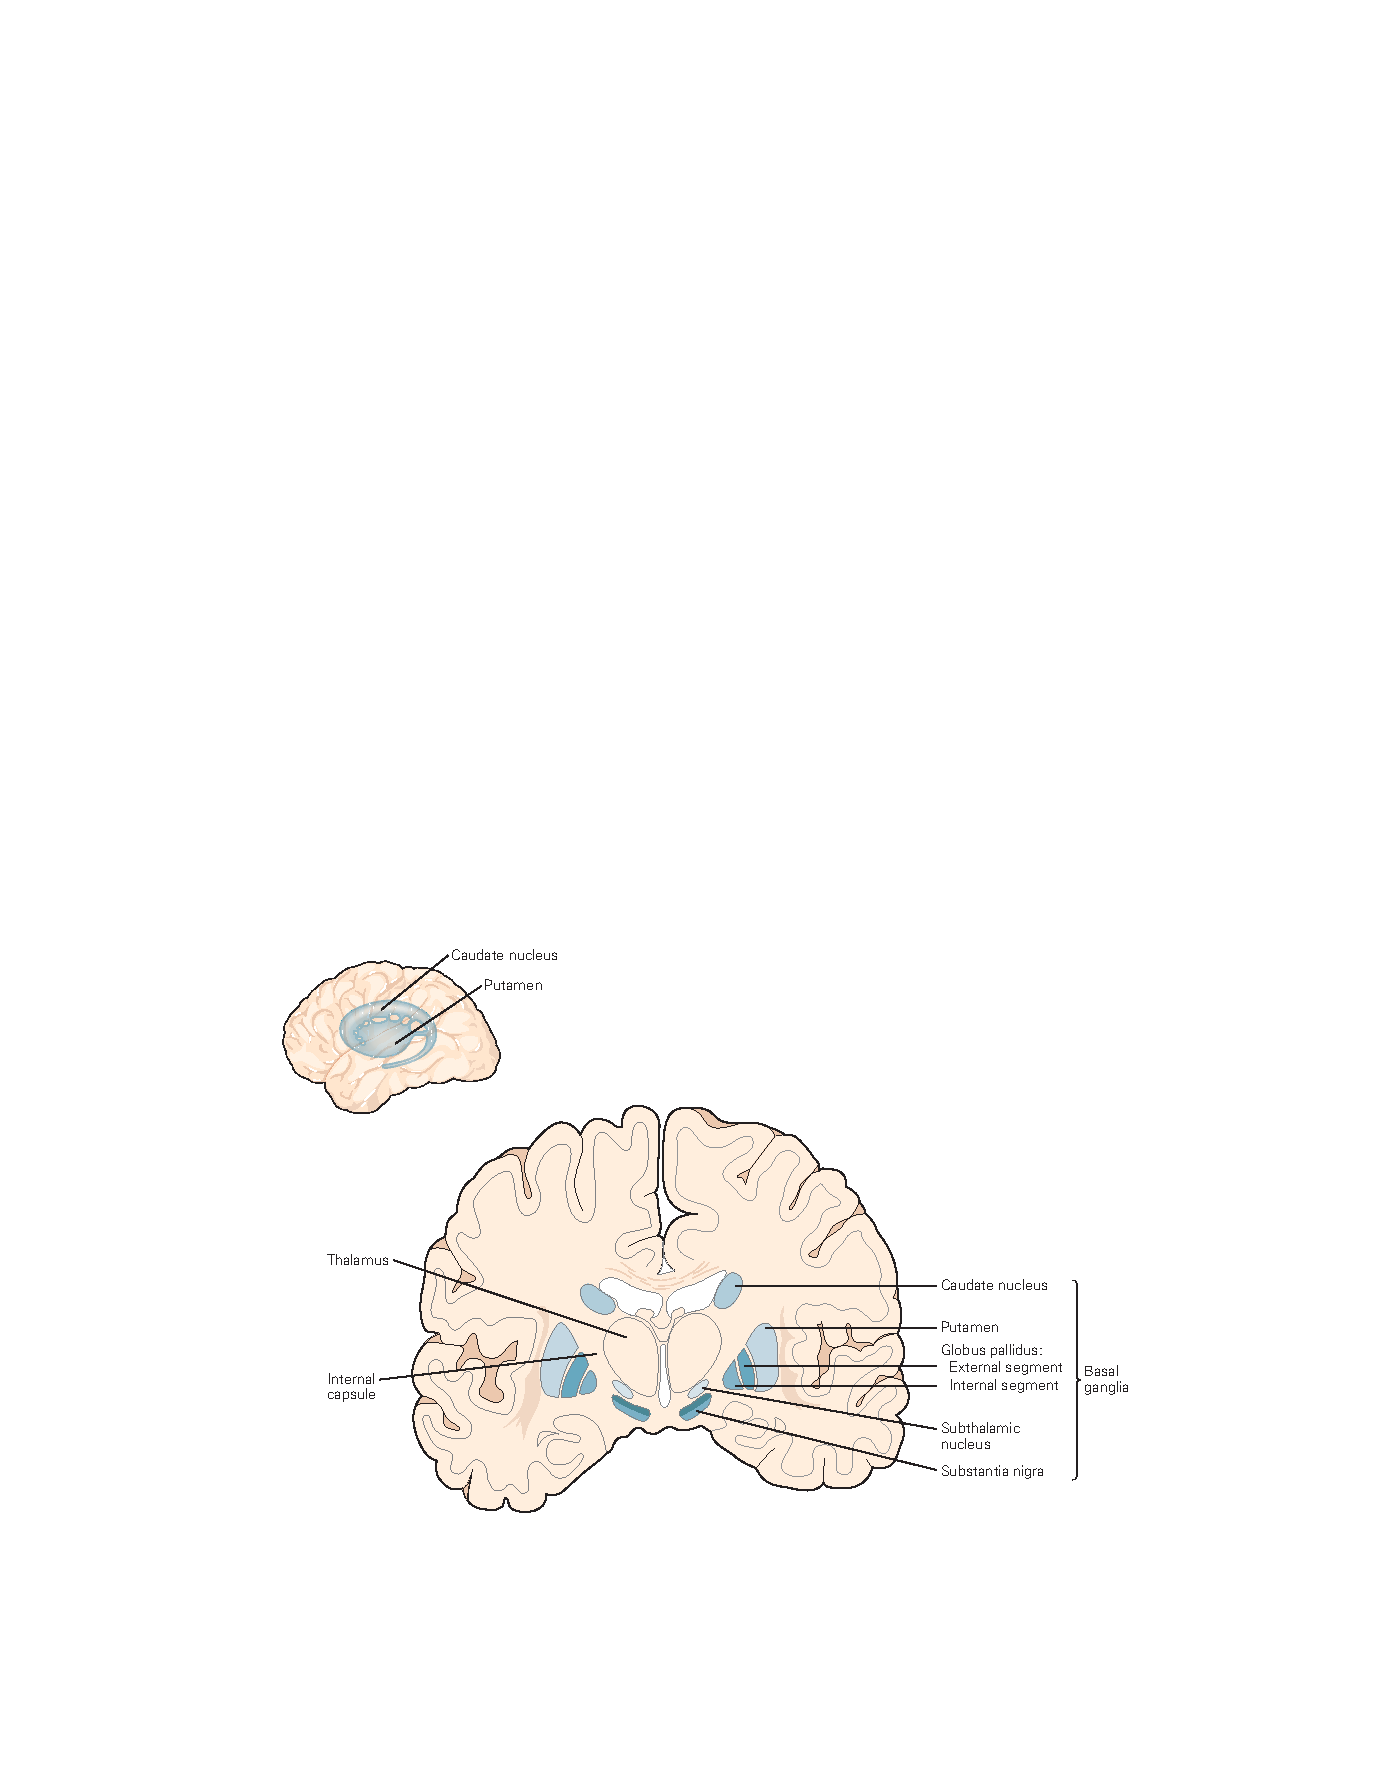
\includegraphics[width=1.0\linewidth]{chap38/fig_38_1}
	\caption{基底神经节和周围结构。
		基底神经节的细胞核位于人脑冠状切面的右侧\cite{nieuwenhuys2007human}。}
	\label{fig:38_1}
\end{figure}



\section{基底神经节网络由三个主输入核、两个主输出核和一个内在核组成}

纹状体(尾状核和壳核的统称;见图~\ref{fig:38_1})、丘脑底核和黑质致密部/腹侧被盖区是基底神经节的三个主要输入核,直接和间接地接收来自结构的信号分布于整个神经轴(图~\ref{fig:38_2})。


\begin{figure}[htbp]
	\centering
	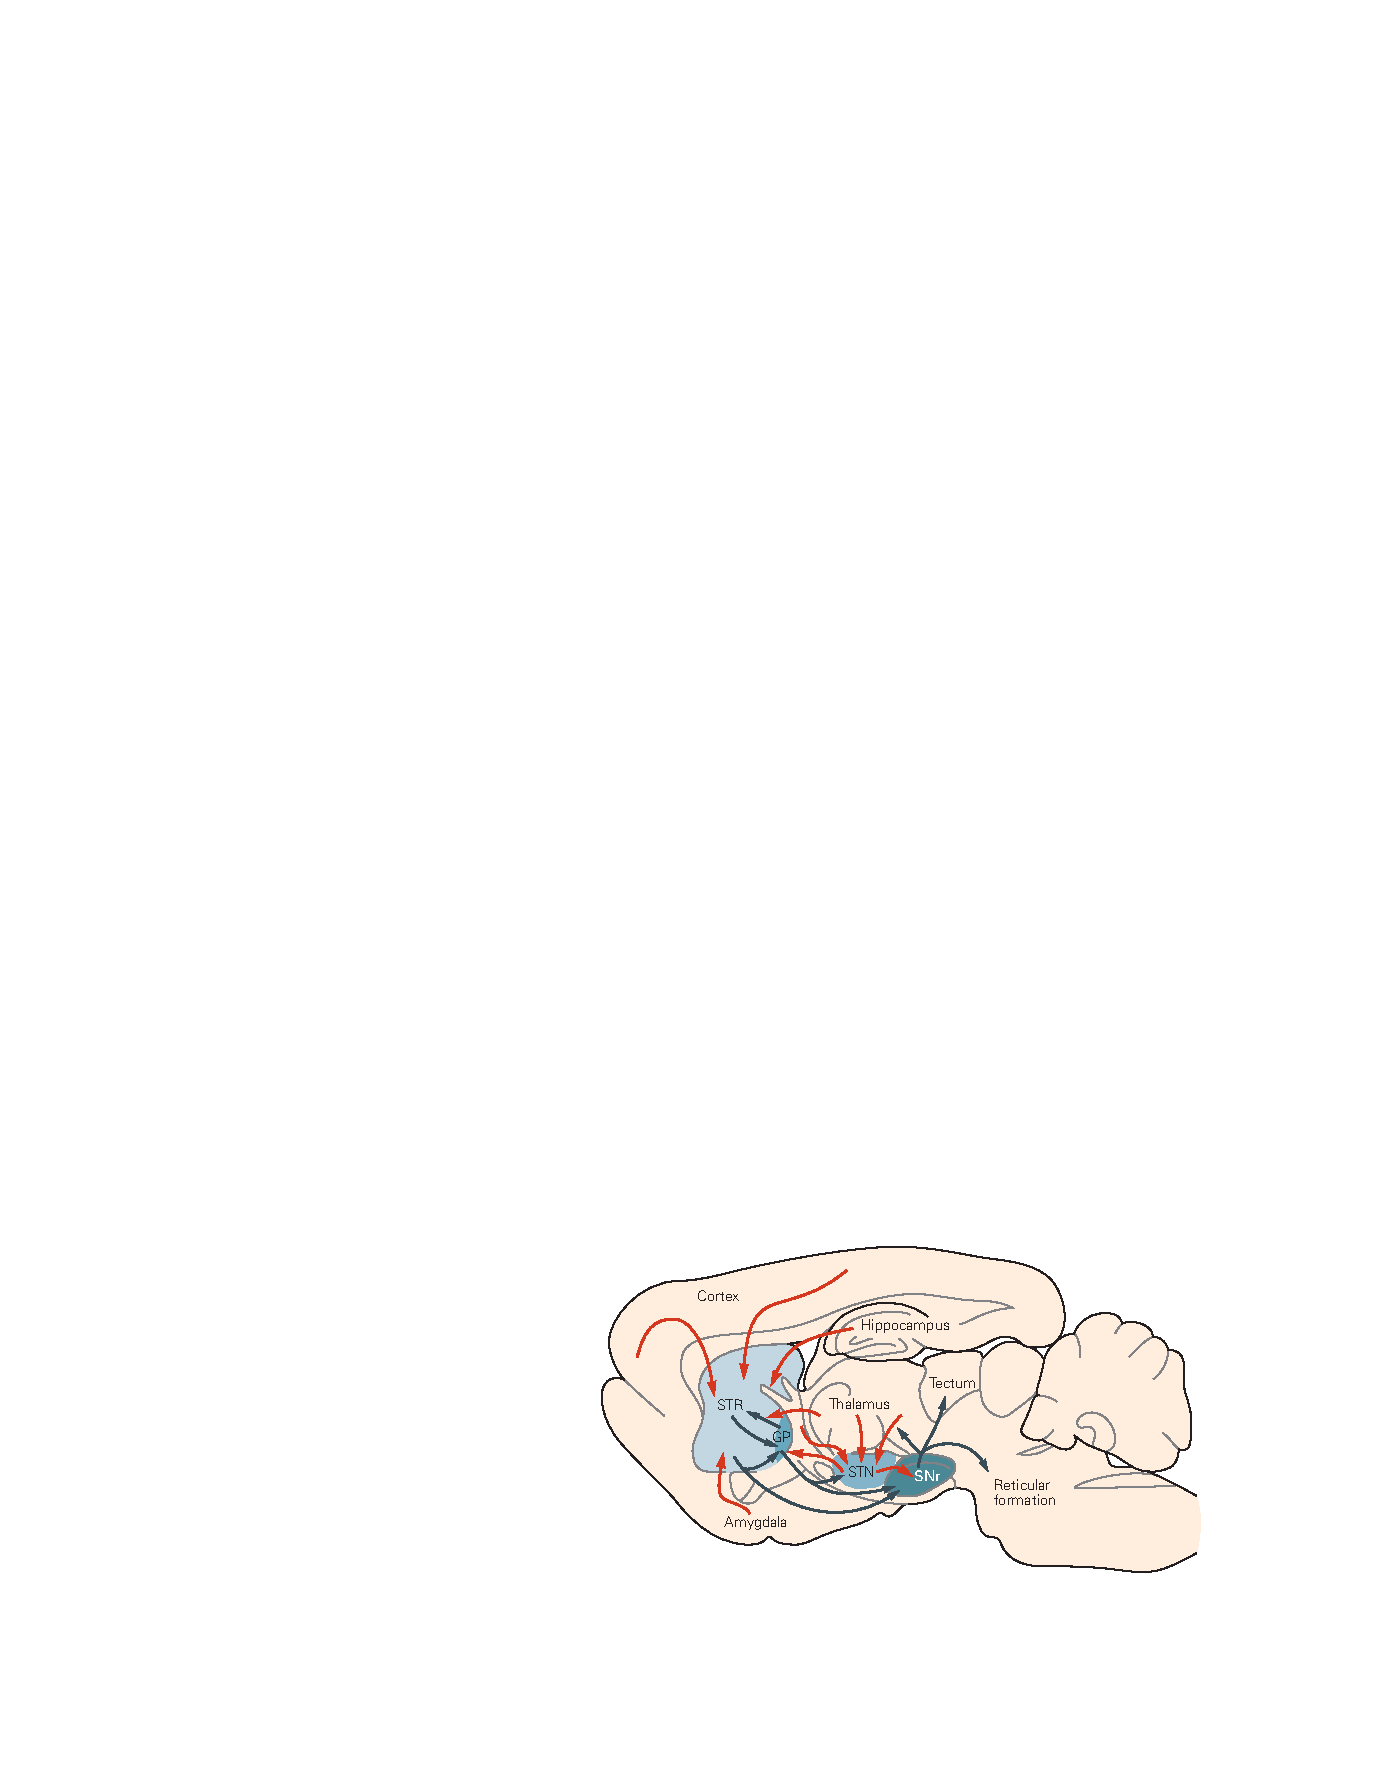
\includegraphics[width=0.78\linewidth]{chap38/fig_38_2}
	\caption{哺乳动物基底神经节的主要输入、内在和输出连接。
		主要输入核是\textit{纹状体}、\textit{丘脑底核}和黑质致密部(未显示)。
		它们直接接收来自丘脑、大脑皮层和边缘结构(杏仁核和海马体)的输入。
		主要输出核是\textit{黑质网状部}和内部苍白球/内脚核(未显示)。
		外部\textit{苍白球}被归类为内在核,因为它的大部分连接都与其他基底神经节核相连。
		结构显示在啮齿动物大脑的矢状图上。
		红色和深灰色箭头分别表示兴奋性和抑制性连接。}
	\label{fig:38_2}
\end{figure}



\subsection{纹状体、丘脑底核和黑质致密部/腹侧被盖区是基底神经节的三个主要输入核}

纹状体是基底神经节中最大的核。
它接收来自大脑皮层和边缘结构的大部分区域的直接输入,包括杏仁核和海马体。
来自脑干感觉运动和动机区域的重要输入通过丘脑间接传递。
在啮齿类动物中,纹状体从大脑皮层和丘脑接收到的接触数量大致相等。
最后,纹状体的重要调节输入来自黑质致密部(多巴胺)、中脑中缝(血清素)和脚桥核(乙酰胆碱)。


纹状体根据输入连接的组织在功能上进行细分,主要是来自大脑皮层的拓扑组织传入。
边缘、联想和感觉运动区域通常沿着腹内侧背外侧连续体被识别。
这种输入的多样性表明,基底神经节从涉及不同动机、情绪、认知和感觉运动过程的大脑区域接收信号,这意味着无论基底神经节在做什么,它们都在为广泛的大脑过程做这件事。


纹状体的另一个结构特征表明,基底神经节对来自功能不同的传入结构的输入执行或多或少相同的操作。
具体来说,在纹状体的每个功能区域内,细胞结构都非常相似。
在所有区域中,抑制性的\textit{$\gamma$-氨基丁酸}能中型棘细胞神经元是主要细胞类型(>90\% 的所有神经元)。
此外,在所有功能定义区域中,根据神经活性肽(物质 P 和强啡肽与脑啡肽)的相对表达或 D1 和 D2 多巴胺受体的表达,中型多刺神经元被分成两个群体,这被认为对积极和 负调节这些神经元中的环磷酸腺苷信号。
这些群体对纹状体的不同传出投射有不同的贡献。
除了这些与其他基底神经节核的远程抑制连接外,中型多刺神经元还会将局部侧枝传送到相邻细胞。
共定位的\textit{$\gamma$-氨基丁酸}能和肽能神经传递提供局部相互抑制和兴奋的影响。
纹状体中其余 5\% 至 10\% 的神经元是纯\textit{$\gamma$-氨基丁酸}能和胆碱能中间神经元,可根据神经化学、电生理学和某些情况下的形态学特征进行区分。
这种局部细胞结构存在于所有功能区域的事实表明,纹状体中的神经元正在对功能不同的传入通路应用相同或相似的计算。


底丘脑核传统上被认为是从纹状体到基底神经节输出核的“间接输出通路”中的重要内部中继(见下文)。
它现在也被认为是基底神经节的第二个重要输入核。
按地形组织的输入不仅来自额叶皮层的大部分,还来自各种丘脑和脑干结构。
底丘脑核是基底神经节中唯一具有兴奋性(谷氨酸能)输出连接的组成部分。
这些投射到输出核和内在的外部苍白球。


黑质致密部/腹侧被盖区包含大量多巴胺能神经元。
这些神经元代表基底神经节的第三个主要输入站,并产生黑质纹状体和中脑边缘/中皮质多巴胺投射。
它们接收来自其他基底神经节核团(纹状体、苍白球和丘脑底)的重要传入连接,但也接收来自脑干中许多结构(例如,上丘、喙内侧被盖区、中缝核、桥足核和臂旁区)的传入连接。
其他传入连接来自额叶皮层和杏仁核。
这种连接模式很重要,因为它表明对多巴胺能神经元最重要的直接影响来自大脑进化上古老的部分(见下文)。


单个多巴胺能神经元具有高度分支的轴突,这些轴突不仅投射到其他基底神经节核团的广泛区域,而且投射到外部结构(例如,额叶皮层、隔区、杏仁核、缰核)。
这表明它们的重要调制信号在整个目标结构中广泛传播。 在纹状体中发现了最高浓度的多巴胺能末端,其中与中型多刺细胞和中间神经元形成突触和非突触接触。
非突触接触的存在导致了所谓的体积传递。
当神经递质从可能远离目标细胞的释放点扩散到大脑的细胞外液时,就会发生这种情况。
因此,体积传递通常比突触神经传递具有更长的时间过程。
在目标结构中部署体积传输进一步证明了多巴胺在目标结构中的影响广泛传播且空间不精确的观点。
不同比例的\textit{$\gamma$-氨基丁酸}能神经元(黑质和腹侧被盖区)和谷氨酸能神经元(腹侧被盖区)有助于这些结构中的局部处理。



\subsection{黑质网状部和内部苍白球是基底神经节的两个主要输出核}

内部苍白球/内脚核是两个主要输出核之一。
它接收来自其他基底神经节核团的输入,并投射到丘脑和脑干中的外部目标。
来自纹状体和外部苍白球的\textit{$\gamma$-氨基丁酸}能输入是抑制性的,而来自底丘脑核的输入是谷氨酸能和兴奋性的。
内部苍白球的神经元本身是\textit{$\gamma$-氨基丁酸}能,具有高水平的强直活性。
在正常情况下,这会对丘脑、外侧缰核和脑干中的目标产生强大的抑制作用。


黑质网状部是第二个主要输出核。
它还接收来自其他基底神经节核团的传入,并提供与丘脑和脑干的传出连接。
抑制性(氨基丁酸能)输入来自纹状体和苍白球(外部),兴奋性输入来自底丘脑。
网状部神经元也是\textit{$\gamma$-氨基丁酸}能的,对部分丘脑和脑干施加强烈的抑制控制,包括上丘、脚桥核以及部分中脑和髓质网状结构。



\subsection{外部苍白球主要是基底神经节的内在结构}

苍白球的大部分连接都与其他基底神经节核团相连,包括来自纹状体的抑制性(\textit{$\gamma$-氨基丁酸}能)输入和来自底丘脑的兴奋性(谷氨酸能)输入,苍白球为所有基底神经节的输入和输出核团提供抑制性传出连接。
这种连接模式表明外部苍白球是内部基底神经节活动的重要调节器。


描述了基底神经节的核心组成部分之后,我们现在将更详细地考虑它们是如何连接的,首先是相互连接,然后是大脑中的外部结构。



\section{基底神经节的内部回路调节组件如何相互作用}

\subsection{基底神经节的传统模型强调直接和间接通路}

\textit{罗杰$\cdot$阿尔宾}及其同事在 1980 年代后期提出了对基底神经节内在回路的一种有影响力的解释(图~\ref{fig:38_3}A)。
在他们的方案中,源自大脑皮层的信号被分配到纹状体中的两个中等多刺输出神经元群。


\begin{figure}[htbp]
	\centering
	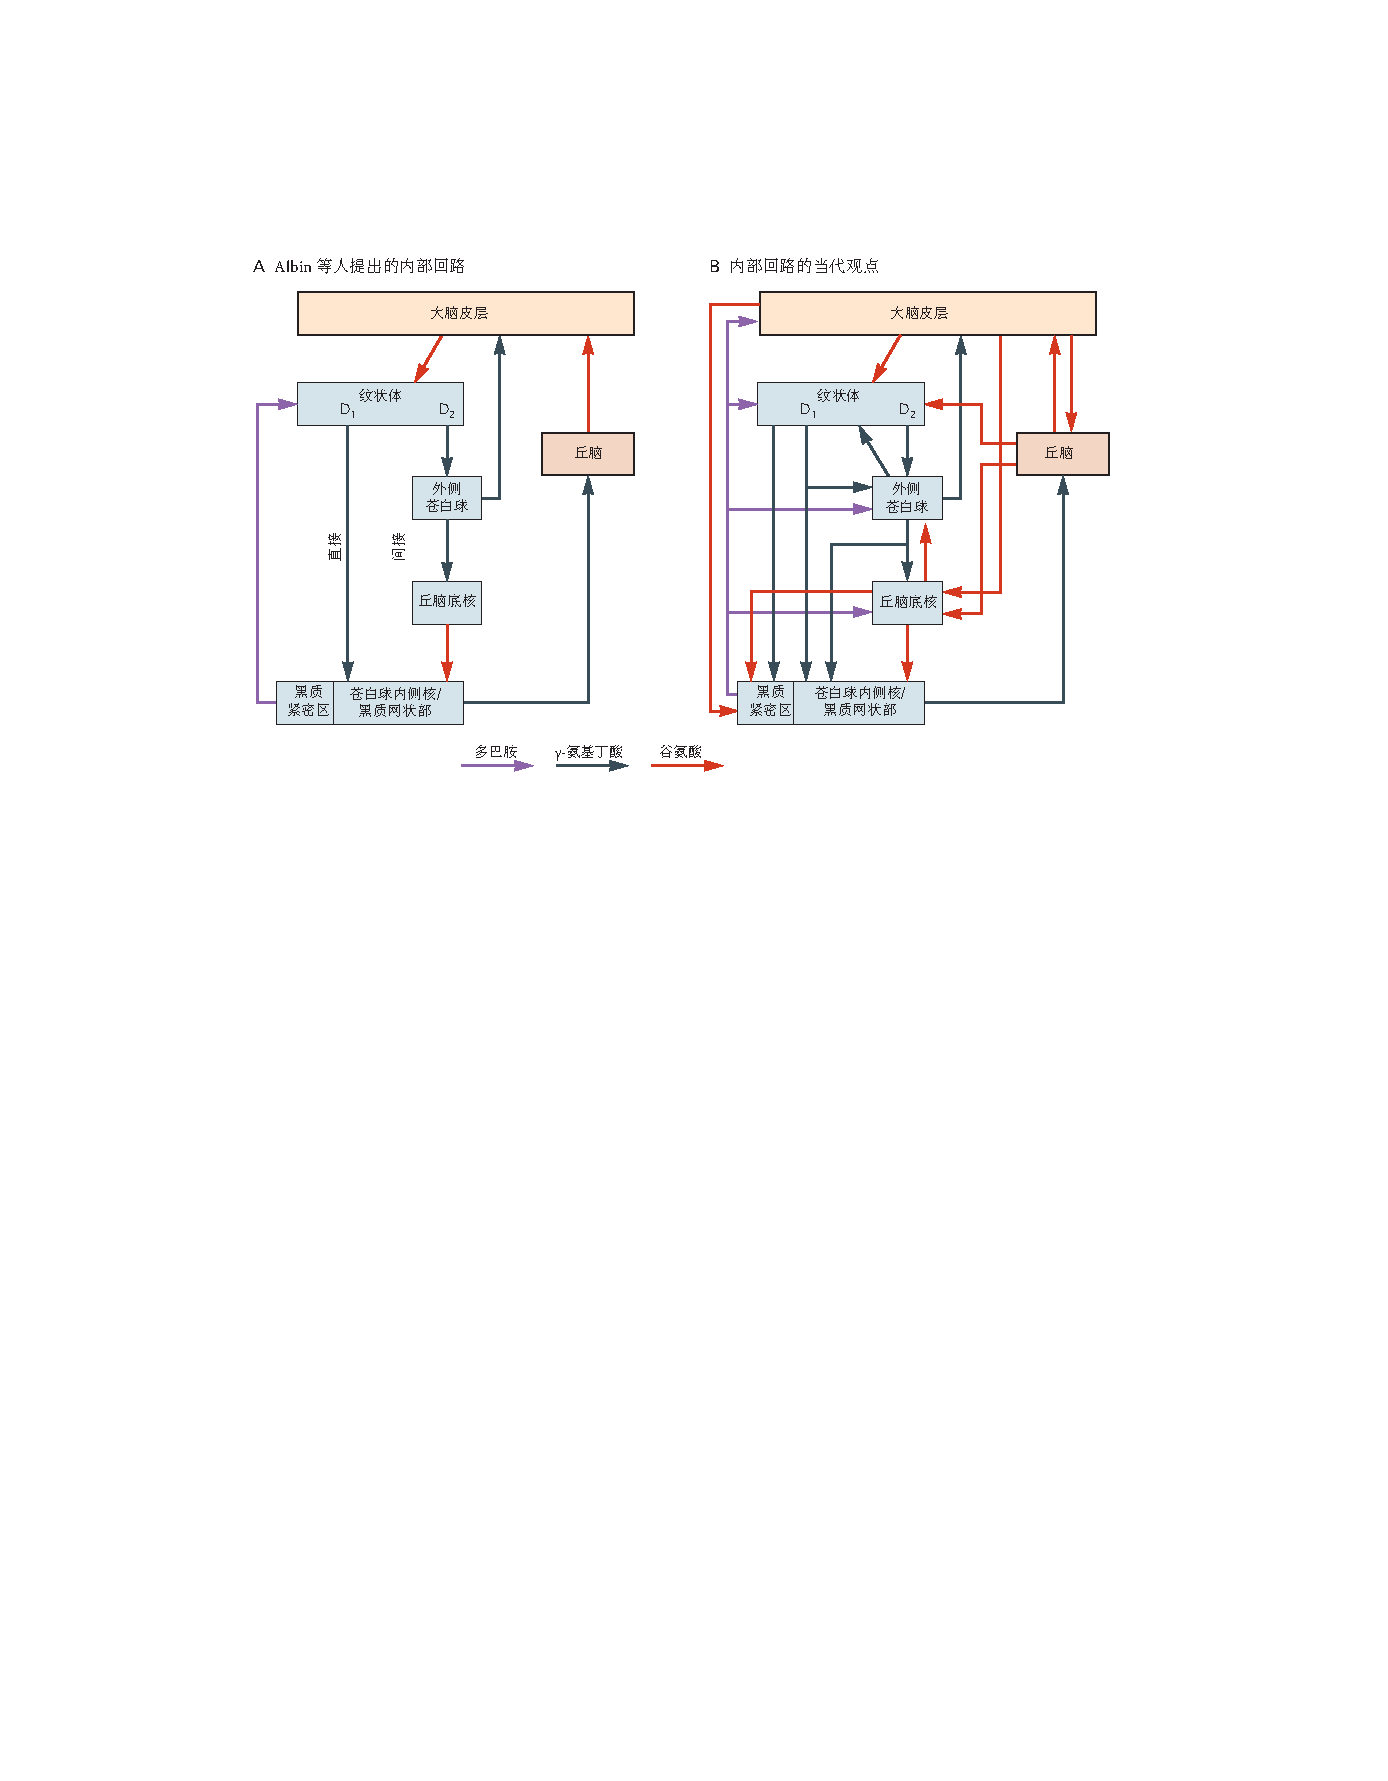
\includegraphics[width=1.0\linewidth]{chap38/fig_38_3}
	\caption{基底神经节内的内在联系。
		\textbf{A.} \textit{罗杰$\cdot$阿尔宾}及其同事(1989)提出了有影响力的提议,其中基底神经节的输出取决于从纹状体到输出核(\textit{苍白球内侧核}和实质性\textit{黑质网状部})的直接通路之间的平衡),它促进行为,以及通过\textit{外侧苍白球}和\textit{丘脑底核}中的中继从纹状体到输出核的间接通路,抑制行为。
		直接和间接投射之间的平衡被认为是由来自\textit{黑质紧密区}的传入多巴胺能信号调节的,作用于差异分布的 D1 和 D2 多巴胺受体。
		\textbf{B.} 最近的解剖学研究揭示了一个相当复杂的组织,其中产生输出的基底神经节输入的转换不太容易预测。}
	\label{fig:38_3}
\end{figure}


含有 P 物质和大量 D1 多巴胺受体的神经元与基底神经节输出核直接抑制接触,即直接通路。
相比之下,含有脑啡肽并主要表达 D2 多巴胺受体的纹状体神经元通过苍白球和丘脑底中的中继(间接通路)与输出核进行兴奋性接触。
基底神经节输出被认为反映了皮层决定的这些抑制性和兴奋性投射之间的平衡,这些投射终止于两个输出结构(内部苍白球和黑质网状部)。
在这个模型中,当直接途径占主导地位时,行为会得到促进,而当间接途径占主导地位时,行为会受到抑制。



\subsection{详细的解剖分析揭示了一个更复杂的组织}

最近的解剖学观察表明,基底神经节的内部回路比最初设想的更复杂(图~\ref{fig:38_3}B)。
主要发现是:
(1)直接通路的中型多刺神经元也为苍白球提供侧支输入; 
(2)除了与底丘脑的传统间接连接外,苍白球神经元还与输出核直接接触,通常与所有三个结构都有分支侧支;
(3)苍白球也投射回纹状体和基底神经节外的结构;
(4)除了与两个基底神经节输出核的前馈连接外,底丘脑核还投射回外部苍白球; 
(5)底丘脑核的主要输入来自基底神经节外部的皮层和皮层下结构。
因此,底丘脑现在被认为是基底神经节的主要输入结构(见上文),而不是固有间接投射中的简单中继。
对基底神经节内这种复杂组织的现代认识表明,不再可能凭直觉判断特定输入如何被基底神经节转化为特定输出。
因此,基底神经节内部回路的计算建模变得越来越重要。


尽管内在回路的整体模式很复杂(图~\ref{fig:38_3}B),但基底神经节组件之间的连接在整个拓扑结构中是有序的。
其中一些投射相对集中(例如,纹状体黑质投射),而其他投射则更为分散(例如,丘脑黑质投射)。
传入结构、纹状体和输出核中神经元的相对数量显著减少表明在基底神经节内处理信息时信息被显著压缩。



\section{基底神经节与外部结构的连接以重入环为特征}

\subsection{输入定义基底神经节的功能区域}

从大脑皮层、边缘结构和丘脑输入到纹状体的功能状态为基底神经节核(边缘、联想和感觉运动)内的功能区域分类提供了基本原理。
然而,传入投射与基底神经节核神经元接触的方式表明存在重要的功能差异。
例如,从大脑皮层和中央外侧丘脑核到达纹状体的轴突似乎很少与许多纹状体神经元接触。
相比之下,来自其他区域(主要是丘脑束旁核)的输入具有轴突,这些轴突与较少的单个纹状体神经元进行多次接触。
与底丘脑核的传入连接,至少来自大脑皮层,也根据边缘、联想和感觉运动分类在地形学上进行组织。
然而,没有证据表明从外部结构到中脑腹侧\textit{黑质紧密区}和\textit{腹侧被盖区}多巴胺神经元的相同类型的精确地形输入。



\subsection{输出神经元投射到提供输入的外部结构}

基底神经节输出神经元投射到丘脑区域(椎板内核和腹内侧核),这些区域投射回基底神经节输入核以及那些为纹状体提供原始输入的皮层区域。
同样,从基底神经节到脑干的输出往往针对那些通过丘脑中线和椎板内核团向纹状体提供输入的区域。
重要的是,从基底神经节输出核到丘脑和脑干的投射也是地形有序的。


最后,基底神经节的许多输出投射被广泛抵押,从而同时联系丘脑、中脑和后脑中的目标。
该组织的功能后果的一个例子是,黑质网状部中与口腔行为相关的神经元子集可以同时影响丘脑/皮层、中脑和后脑特定区域的活动,这些区域在产生口语行为。



\subsection{重入环是基底神经节回路的基本原理}

与基底神经节的输入投射、内在连接和输出相关的空间拓扑为\textit{加勒特$\cdot$亚历山大}及其同事在 1989 年提出的有影响力的组织原则提供了基础。
大脑皮层和基底神经节之间的连接可以看作是一系列可重入平行 突出的、部分分离的皮层-纹状体-黑质-丘脑-皮层环或通道(图~\ref{fig:38_4})。
因此,来自大脑皮层不同功能区域(例如,边缘、联想、感觉运动)的投射的一个重要组成部分与基底神经节输入核的特定区域进行排他性接触。
这种区域分离在整个内部回路的前向投影中得到保持。
来自基底神经节输出核中代表的功能区域的聚焦输出信号通过适当的丘脑转发器返回到提供原始输入信号的皮层区域。


\begin{figure}[htbp]
	\centering
	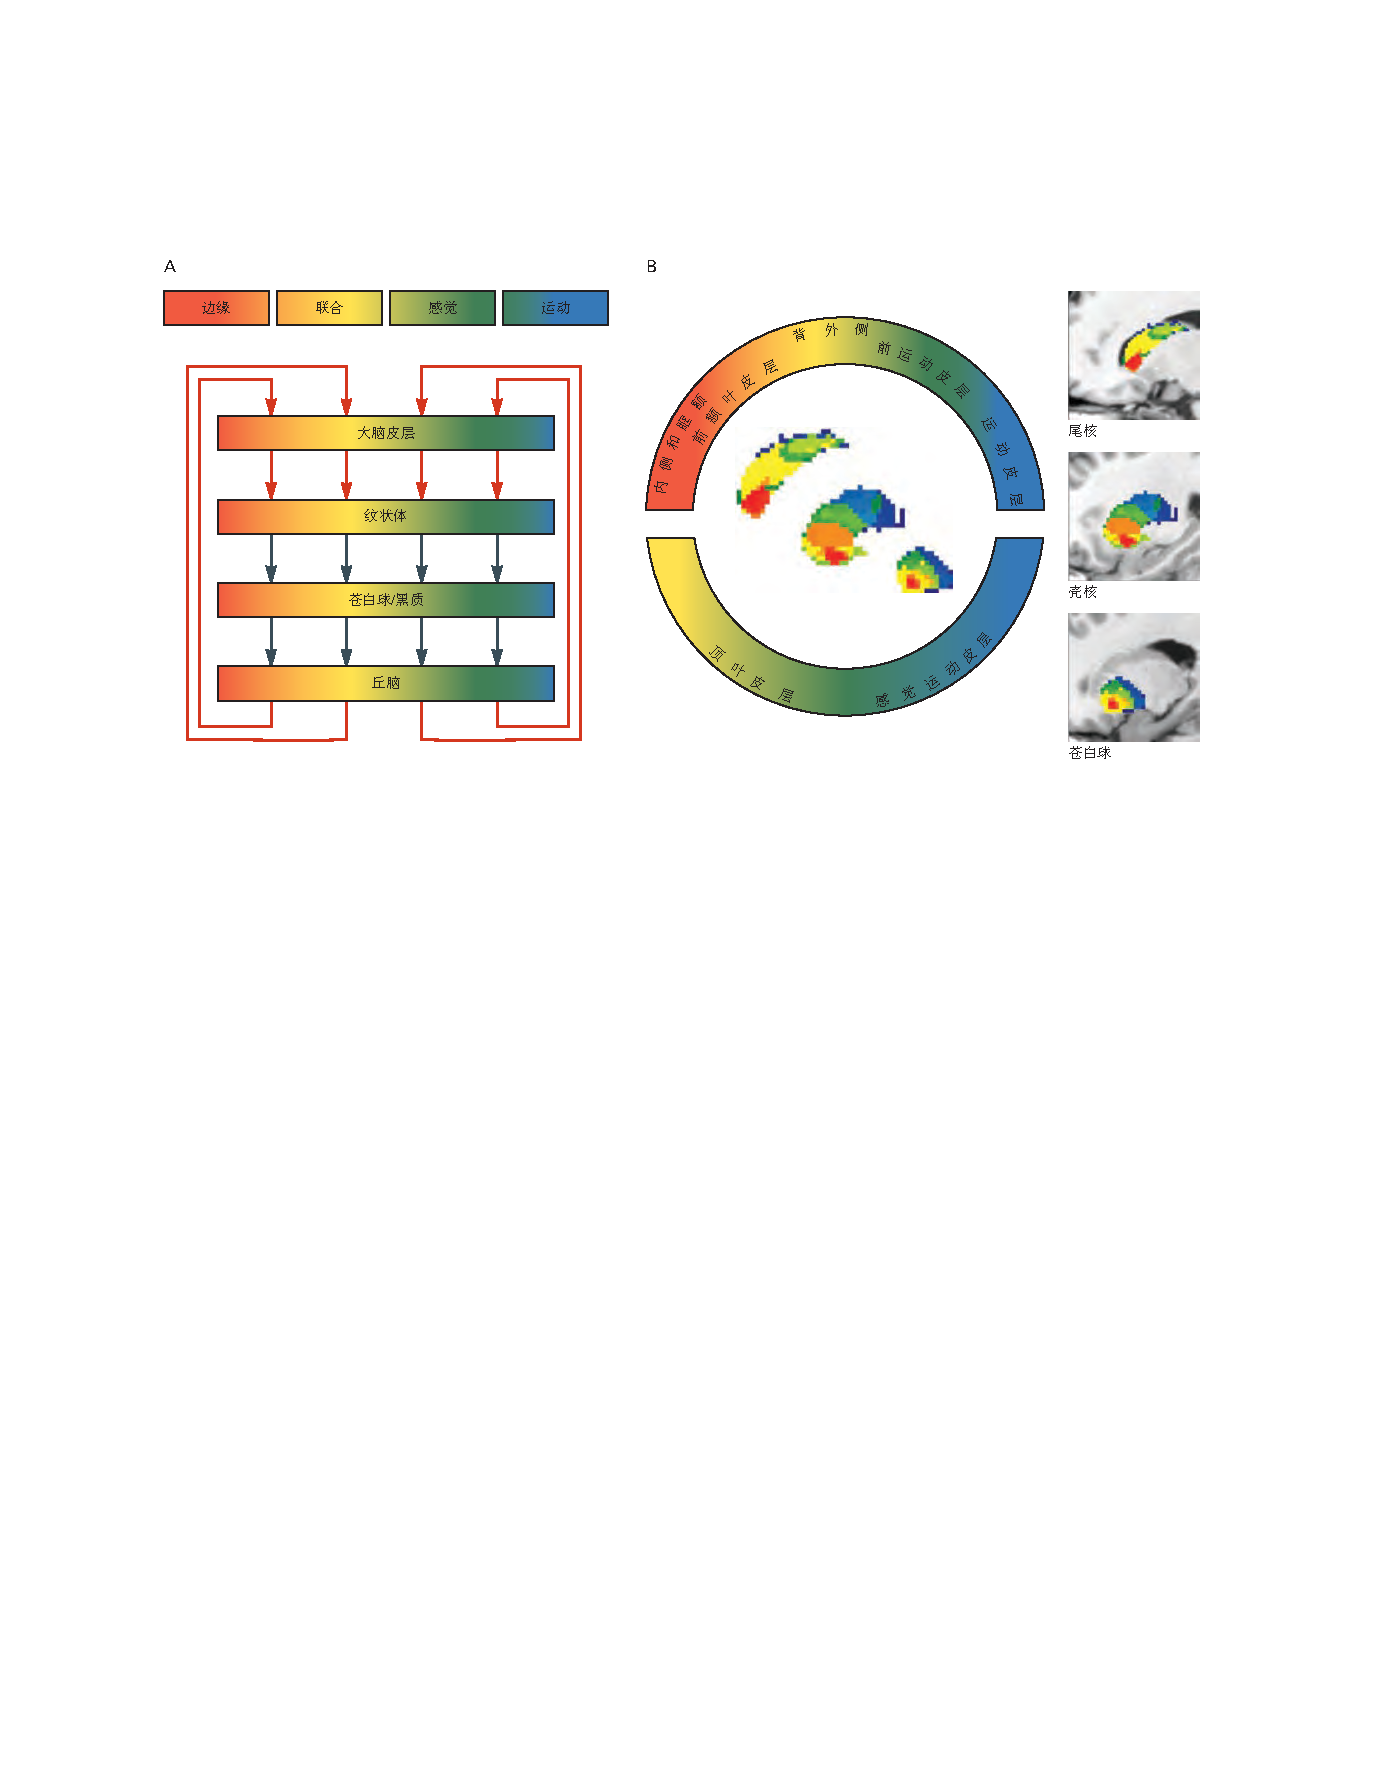
\includegraphics[width=1.0\linewidth]{chap38/fig_38_4}
	\caption{基底神经节和大脑皮层之间的连接。
		\textbf{A.} 大脑皮层和基底神经节之间的连接可以看作是一系列平行投射的、大部分分离的环路或通道。
		在大脑皮层水平代表的功能区域在整个基底神经节核团和丘脑中继中得到维持。
		然而,对于每个循环,皮层、基底神经节和丘脑中的中继点提供了循环内部活动被循环外部信号修改的机会。
		红色和深灰色箭头分别代表兴奋性和抑制性连接。
		\textbf{B.} \textit{尾核}、\textit{壳核}和\textit{苍白球}中人类额叶皮层连通性的空间分离的头端-尾端梯度。
		颜色编码的环表示矢状面上的大脑皮层区域\cite{draganski2008evidence}。}
	\label{fig:38_4}
\end{figure}


通过基底神经节的平行投射折返环的概念已扩展到它们与脑干中的感觉运动和动机结构的连接,包括上丘、导水管周围灰质、脚桥脑和臂旁核。
这意味着通过基底神经节的折返环结构一定早于大脑皮层的进化扩张。
一个重要的区别是,对于皮层环路,丘脑转发器位于环路的输出侧,而对于皮层下环路,丘脑转发器位于输入侧(图~\ref{fig:38_5})。
需要进一步的工作来测试来自不同脑干结构的投射,当它们通过丘脑和基底神经节中继时,是否在功能上是不同的通道。


\begin{figure}[htbp]
	\centering
	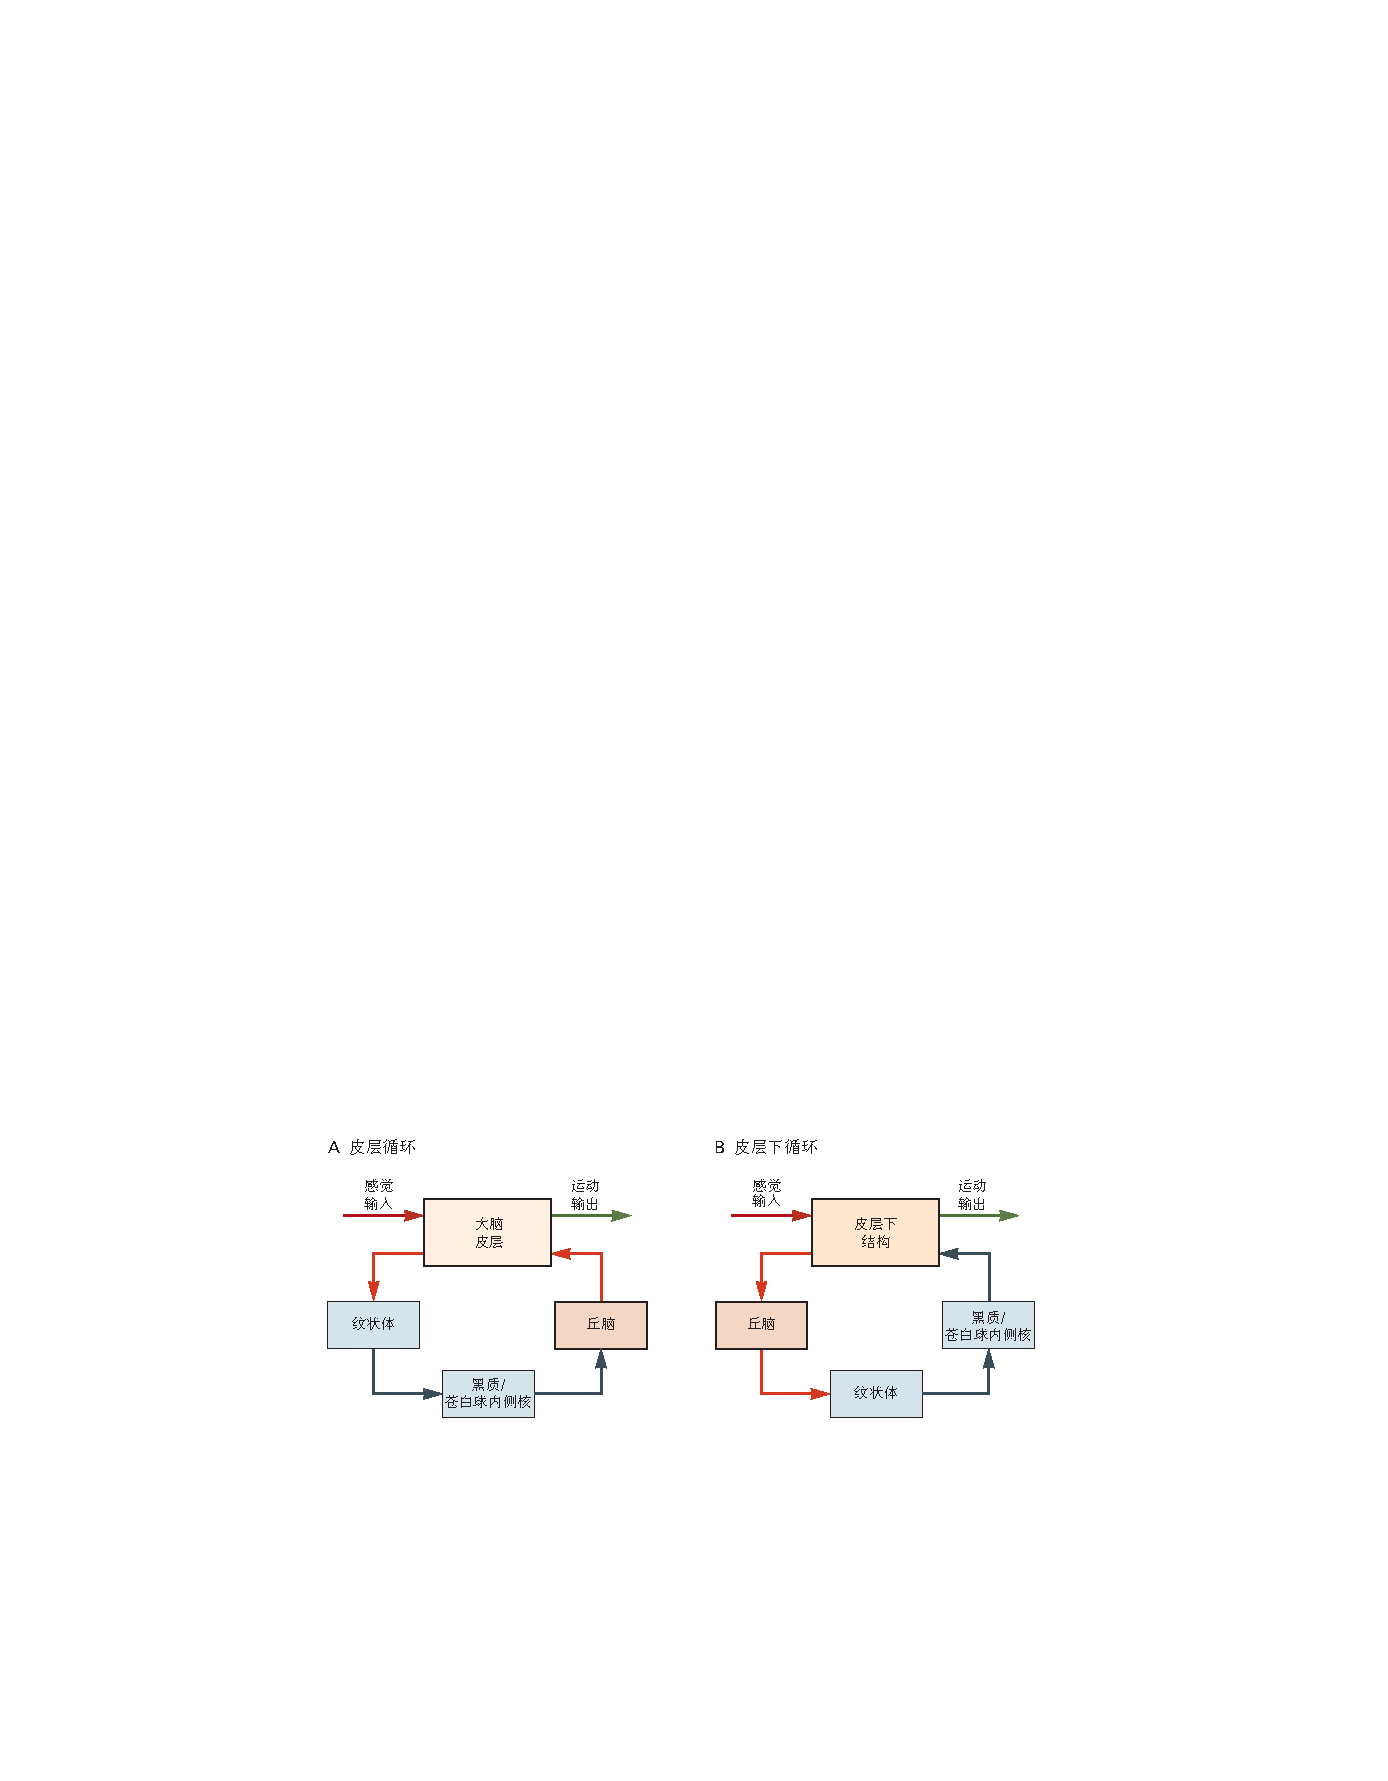
\includegraphics[width=0.87\linewidth]{chap38/fig_38_5}
	\caption{皮层和皮层下感觉运动环路穿过基底神经节。
		\textbf{A.} 对于皮层环路,丘脑转发器的位置在环路的返回臂上。
		\textbf{B.} 在所有皮层下回路的情况下,丘脑转发器的位置在回路的输入侧。
		红色表示主要是兴奋区域和连接,而深灰色表示抑制区域和连接。}
	\label{fig:38_5}
\end{figure}


总之,部分分离的折返环组织是表征基底神经节与外部结构之间连接的主要特征之一。
这种连接模式为了解基底神经节核团在整个大脑功能中所起的作用提供了重要线索。
然而,在这一点上,重要的是不要将可重入循环架构视为由一系列独立且隔离的功能通道组成。
在循环中的每个节点或中继点(例如,在皮层、输入核、输出核和丘脑中),循环内的信息流有机会被来自循环外的信息修改(参见下面关于强化学习的部分)。


在本章开头,我们指出行为是神经网络中信号处理的涌现属性。
指定了基底神经节的系统级网络后,我们现在考虑在该系统内处理的信号。



\section{生理信号为基底神经节的功能提供了更多线索}

\subsection{纹状体和丘脑底核主要接收来自大脑皮层、丘脑和中脑腹侧的信号}

纹状体从大脑皮层和丘脑接收到的信号通过兴奋性谷氨酸能神经传递进行传递。
当中型多刺神经元接近静息电位时,这些快速、阶段性活跃的兴奋性输入主要由\textit{$\alpha$-氨基-3-羟基-5-甲基异恶唑-4-丙酸}和红藻氨酸受体介导;
当神经元去极化时,\textit{N-甲基-D-天冬氨酸}受体发挥更大的作用。
来自大脑皮层和丘脑的谷氨酸能输入也会影响纹状体中间神经元。


重要的是要认识到这些信号来自外部结构,这些结构同时产生了广泛的行为选择。
由于这些选项不能同时表达,因此这些对基底节的输入被认为是相互竞争的。
纹状体的另一个重要信号是产生行为反应外部结构的输出活动\textit{传出副本}。
例如,背外侧纹状体的感觉运动区域接收来自运动皮层轴突的侧支纤维,这些轴突向脊髓发送信号。


来自腹侧中脑的多巴胺能输入对纹状体神经元活动的影响很复杂,有许多相互矛盾的结果。
在某种程度上,这是由于在切片和麻醉准备中唤起正常输入活动模式的问题。
然而,最近在警觉、活跃的动物身上的光遗传学技术的发展使研究人员能够以时间控制的方式记录和操纵多巴胺信号到纹状体。
因此,目前的证据表明,多巴胺可以增加纹状体中的信噪比,增强强外部输入的影响,同时抑制弱输入。
有进一步的证据表明,多巴胺可以增加直接通路中多刺神经元的兴奋性,同时降低间接通路中多刺神经元的兴奋性。


最后,多巴胺输入对于谷氨酸能输入到来自皮层和丘脑的纹状体中型多刺神经元的长期增强和长期抑制都是必需的。
后一点对于基底神经节在强化学习中所起的作用具有重要意义(见下文)。
多巴胺还可以影响\textit{$\gamma$-氨基丁酸}能和胆碱能中间神经元的活性。
尽管在解剖学上具有重要意义,但对血清素能输入到基底神经节的作用知之甚少。


输入到纹状体的主要外部来源也为底丘脑核提供平行输入。
因此,底丘脑接收来自大脑皮层、丘脑和脑干的时相兴奋性(谷氨酸能)信号。
皮层激活后,丘脑底的短潜伏期兴奋作用被认为是通过这些“超直接”连接介导的,而较长潜伏期的抑制作用更可能来自其他基底神经节核团的间接抑制输入,主要是外部苍白球 。
下丘脑接收来自脑干(例如,上丘)的短潜伏期兴奋性感觉输入;
它还受多巴胺能、血清素能和胆碱能调节输入的影响。



\subsection{腹侧中脑多巴胺神经元接收来自外部结构和其他基底神经节核的输入}

传入中脑腹侧多巴胺能神经元的传入信号来自各种自主、感觉和运动区域,并在一系列时间尺度内运作。
例如,位于黑质外侧的神经元接收来自皮层和皮层下感觉运动区域的短潜伏期兴奋性输入,而更多位于内侧的神经元在较长时间尺度上接收来自下丘脑的短潜伏期感觉信号和自主神经相关输入。


对多巴胺能神经元的重要抑制控制是由\textit{$\gamma$-氨基丁酸}能神经元行使的,既有局部的也有远离区域的,如头内侧被盖。
然而,多巴胺能神经元的最密集输入是来自纹状体和苍白球的抑制性输入以及来自底丘脑核的兴奋性信号。
中脑中缝核提供重要的调节性血清素输入,而脚桥核和外侧背侧被盖核均提供胆碱能和谷氨酸能输入。
关于多巴胺能神经元的广泛传入信号的一个重要功能问题是,多巴胺是执行高度整合的角色,还是执行在不同时间由许多不同系统访问的基本功能。



\subsection{去抑制是基底神经节输出的最终表达}

基底神经节通过抑制和去抑制的基本过程对外部结构产生影响(图~\ref{fig:38_6})。
基底神经节输出核中的\textit{$\gamma$-氨基丁酸}能神经元通常具有高强直放电率(40–80 赫兹)。
这种活动确保丘脑和脑干的目标区域保持在严格和持续的抑制控制下。


\begin{figure}[htbp]
	\centering
	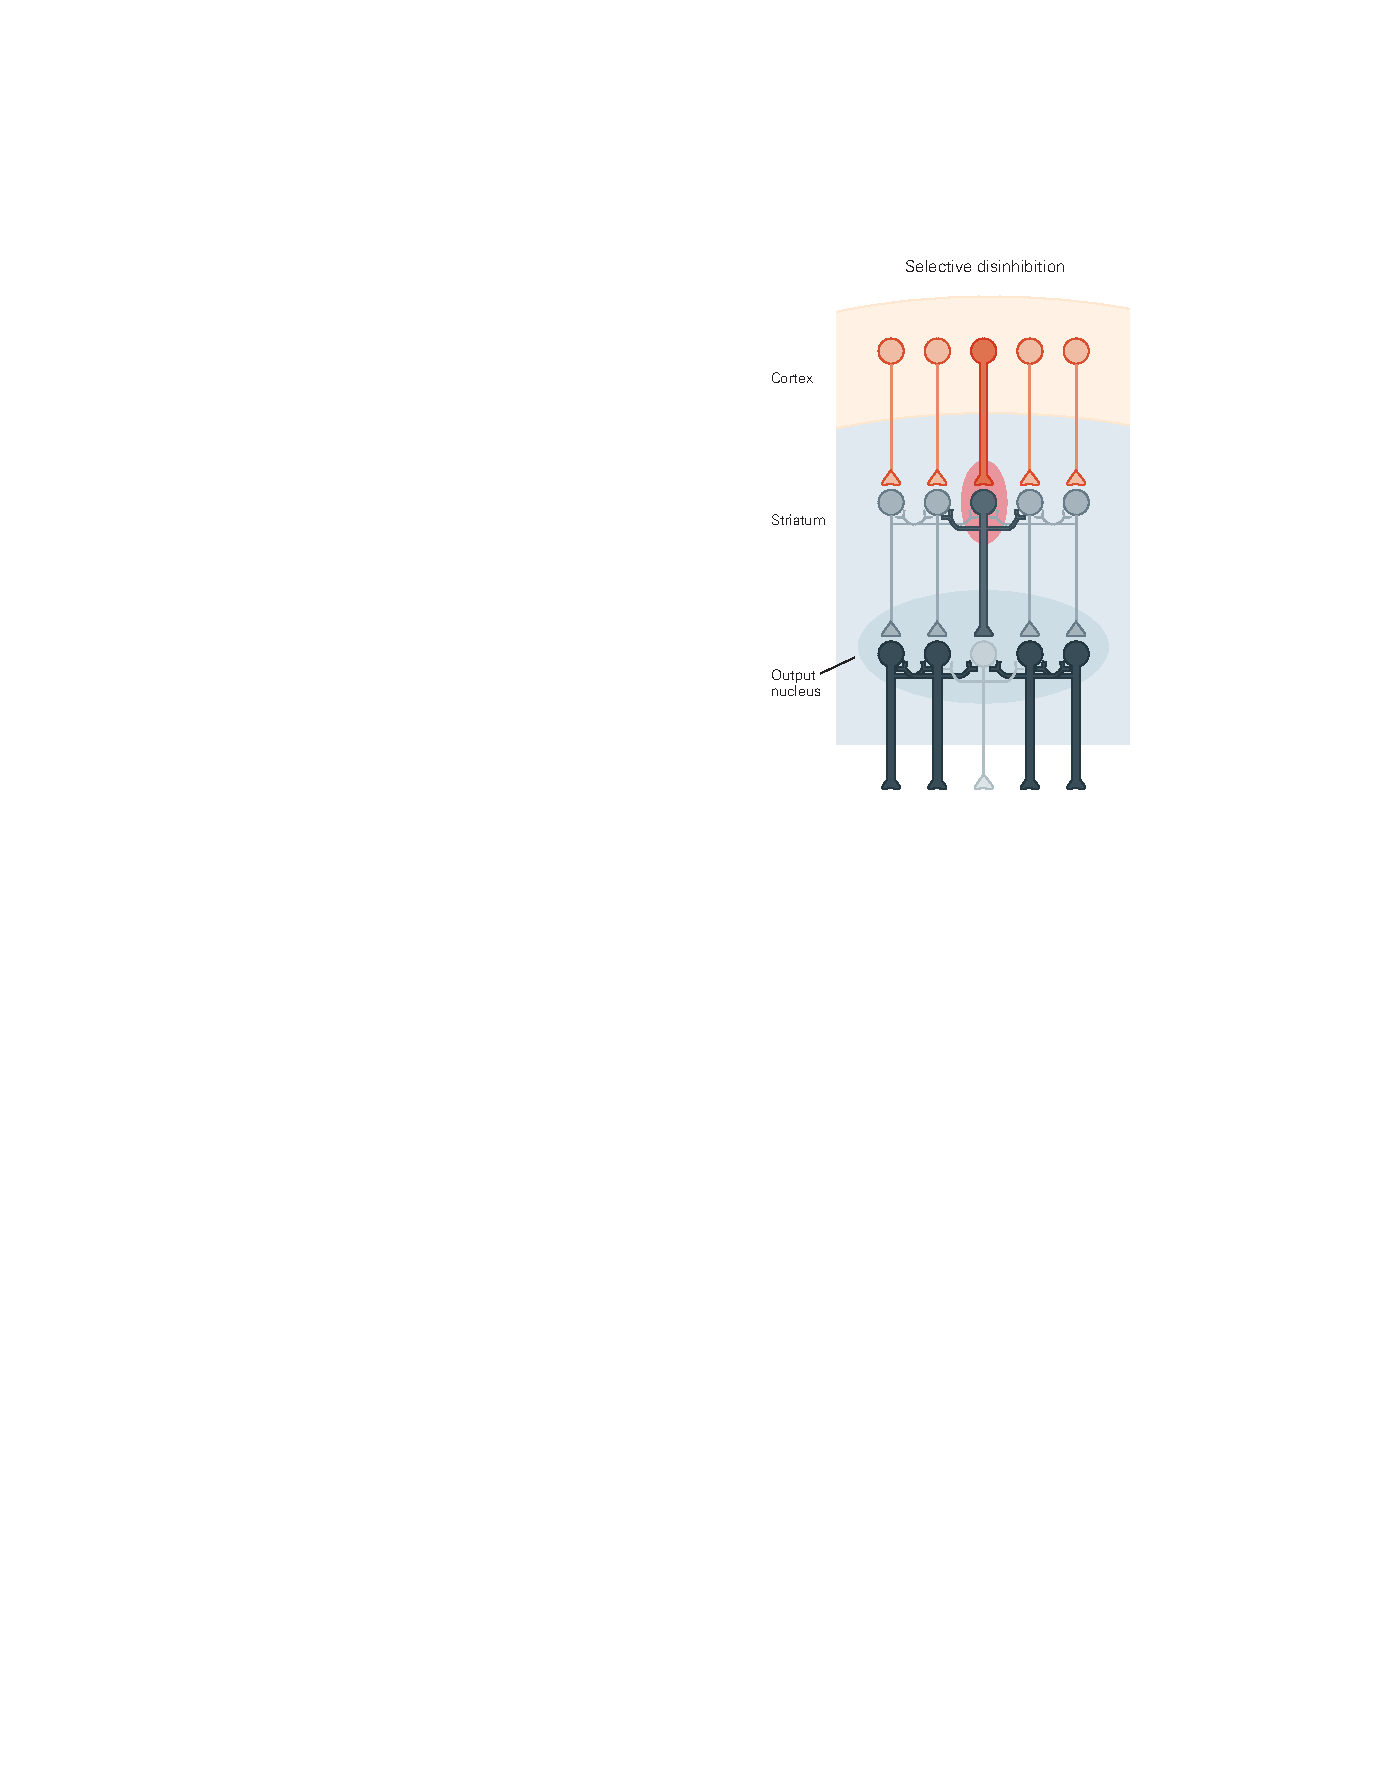
\includegraphics[width=0.45\linewidth]{chap38/fig_38_6}
	\caption{该图说明了在基底神经节输出核水平上进行选择的原理。
		在整个图中,竞争通道内的相对活动水平由投影的厚度表示,为了清楚起见,省略了间接通路和通过丘脑的环路返回连接。
		纹状体的竞争输入之一(中间那个)比它的竞争者更活跃。
		直接抑制途径中的相对活动(此处显示)差异抑制输出核内不同通道中的活动。
		因为输出核神经元也具有抑制性和强性活性,所以所选通道将是来自纹状体的抑制输入最强的通道。
		在未选择的通道上保持强直抑制输出。
		这种在输出核水平上运行的选择性去抑制机制意味着选择将成为整个可重入网络的涌现特性。
		对选定的外部目标解除抑制将使他们能够指挥运动,而非选定的目标仍然受到抑制并且无法影响行为。 红色:兴奋; 灰色:抑制。}
	\label{fig:38_6}
\end{figure}


从外部结构到纹状体的集中兴奋性输入可以对输出核神经元的亚群施加集中抑制(通过直接通路\textit{$\gamma$-氨基丁酸}能抑制连接介导)。
这种抑制输出的集中减少有效地从正常抑制控制中释放或去抑制丘脑(例如,腹内侧核)和脑干(例如,上丘)中的目标区域。
这种强直抑制的突然释放允许目标区域的活动影响行为输出,在中脑上丘的情况下是引起扫视眼球运动。


基底神经节结构内的信号模式提供了对这些网络的整体功能特性可能是什么的重要见解(见下文)。
在考虑脊椎动物大脑的进化史时,对基底神经节可能的核心功能的进一步限制也变得明显。



\section{在整个脊椎动物进化过程中,基底神经节一直高度保守}

哺乳动物基底神经节与系统发生学上古老的脊椎动物(例如七鳃鳗)中发现的基底神经节之间的详细比较发现它们的各个组成部分、内部组织、来自外部结构(皮层/大脑皮层和丘脑)的输入以及 他们的输出核。
例如,在七鳃鳗中观察到来自纹状体中型多刺神经元的直接和间接通路。
类似地,在七鳃鳗内部苍白球和黑质网状部中存在具有强健活性的\textit{$\gamma$-氨基丁酸}能输出神经元。
基底神经节神经元的神经递质和膜特性在进化上的古代和现代物种中也非常相似。


这种高度的形态学和神经化学保护意味着基底神经节回路的结构和操作已经保留了 5 亿多年。
因此,基底神经节是所有脊椎动物共有的大脑结构的重要组成部分。
请记住,在特定神经网络中处理的特定信号模式会产生一种功能,脊椎动物物种中基底神经节结构的保护对其整体功能施加了额外的重要限制。
无论基底神经节在进化上古老的物种中进化来解决什么计算问题,同样的问题很可能保持不变并面临包括人类在内的所有脊椎动物物种。


到目前为止,我们已经确定了基底神经节形态、连接结构、信号处理和进化的特征,这些特征为基底神经节在整体大脑功能中的作用提供了潜在的见解。
因此,拟议的功能必须与连接外部结构与基底神经节的主要环状结构以及在基底神经节核的边缘、联想和感觉运动区域共享的内部回路一致,并且它们必须由所有人共享 脊椎动物物种。
考虑到这些限制,我们现在考虑基底神经节可以支持的功能特性。



\section{\textit{动作选择}是基底神经节研究中反复出现的主题}

尽管有许多建议表明基底神经节涉及广泛的功能,包括感知、学习、记忆、注意力、运动功能的许多方面,甚至镇痛和癫痫发作抑制,但越来越多的证据表明这些核在各种选择过程。
因此,在大量关于基底神经节的文献中,反复提到这些核参与动作选择和强化学习的基本大脑功能。
在本节和下一节中,我们将评估这些核心流程与上述功能限制的一致性程度。



\subsection{所有脊椎动物都面临从多个竞争选项中选择一种行为的挑战}

脊椎动物是多功能生物:
它们必须保持能量和体液平衡、抵御伤害并进行生殖活动。
大脑的不同区域并行运作以提供这些基本功能,但必须共享有限的运动资源。
\textit{谢林顿}的“最终通用汽车路径”意味着不可能同时说话和喝酒。
因此,所有脊椎动物不断面临的一个基本选择问题是确定应允许哪个功能系统在任何时间点指导行为输出。
这是一个在 5 亿年的进化史过程中没有发生实质性变化的问题。
这段时间发生的变化是不同物种为实现生存和繁殖的核心功能而进化的行为选择。
因此,脊椎动物大脑中必须有一个系统可以在同时竞争行为表达的动机系统之间进行裁决。


脊椎动物多模式感觉系统中也出现了类似的选择问题。
视觉、听觉、嗅觉和触觉系统不断面临多种外部刺激,每一种刺激都可能引发与其他刺激不相容的运动(例如,定向/接近、回避/逃避)。
因此,当务之急是选择将成为注意力和直接运动焦点的刺激。
问题是在任何时候应该让哪种刺激进入运动系统。
选择性注意为这个问题提供了有效的解决方案,使其成为脊椎动物大脑功能的一个基本特征。


总之,尽管在不同物种中竞争行为表达的感觉、动机、认知和运动系统的范围、力量和复杂性发生了巨大的进化变化,但选择的基本计算问题仍然没有改变。
而且,如果基底神经节为选择问题提供了一个通用的解决方案,那么脊椎动物大脑进化中的高度结构和功能保守性就有望实现。



\subsection{动机、情感、认知和感觉运动处理需要选择}

\textit{威廉$\cdot$詹姆斯}在他的《心理学原理》中观察到:“选择是建造我们精神之船的龙骨。” 
在这个陈述中,他告诉我们动机、情感、认知、感知和运动表现的神经系统在某个阶段需要咨询一种机制,该机制可以在并行处理但不兼容的选项之间进行选择(图~\ref{fig:38_7})。
因此,重要的是基底神经节核内的内在回路在边缘、联想和感觉运动区域是相似的。


\begin{figure}[htbp]
	\centering
	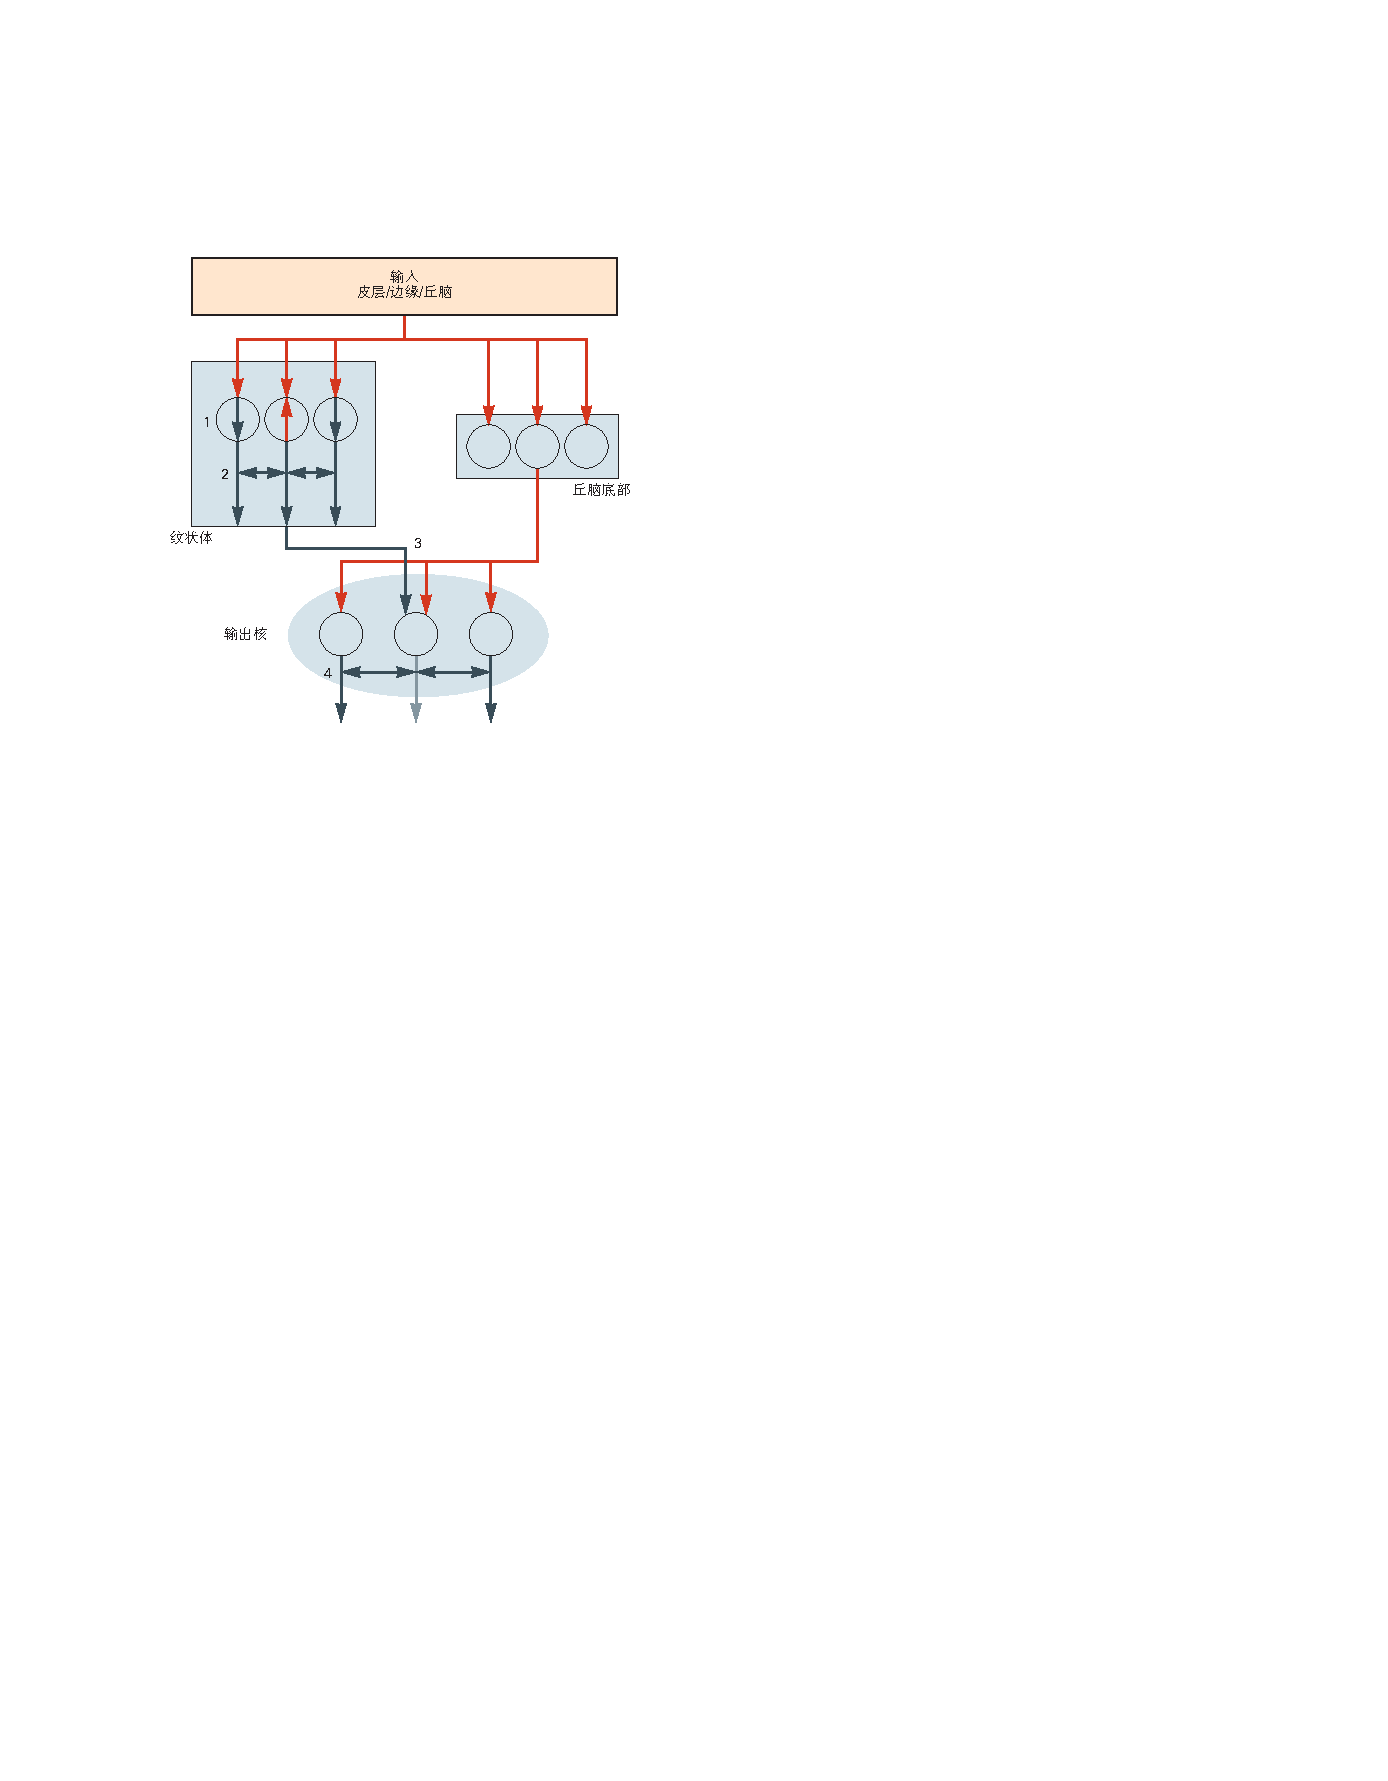
\includegraphics[width=0.65\linewidth]{chap38/fig_38_7}
	\caption{基底神经节中促进选择的合作机制。
		1. 由于皮层和一些丘脑输入与单个纹状体神经元的接触相对较少,因此需要大量足够同步的兴奋性输入来使中等多刺神经元的膜去极化到足以激发动作电位的“向上”状态。
		这种机制可以看作是一种输入过滤器,用于排除较弱或生物学意义较小的竞争者。
		纹状体神经元中的内部箭头表示“向上”(红色)和“向下”(灰色)状态。
		2. 纹状体多刺神经元之间的局部\textit{$\gamma$-氨基丁酸}能和肽能抑制性络脉以及中间神经元的长程抑制作用应导致高度活化的纹状体元件抑制相邻更弱活化通道的活动。
		3. 来自纹状体的集中抑制与来自底丘脑的更弥漫性兴奋的结合将降低选定通道的活动并增加基底神经节输出核中非选定通道的活动。
		纹状体和底丘脑神经元之一的输出已被说明以说明这一点。
		4. 输出核神经元之间的局部抑制性络脉应进一步加剧抑制通道和非抑制通道之间的差异。}
	\label{fig:38_7}
\end{figure}


基底神经节回路中的这种重复表明相同或相似的计算过程适用于来自非常不同的功能来源的输入。
因此,这种重复的回路将能够解决边缘区域中高层动机目标之间的竞争;
中央联想区域中不相容的认知表征之间的竞争;
以及解决了横向感觉运动区域中不相容的感觉和运动选项之间的竞争。



\subsection{基底神经节的神经结构可供选择}

在过去 40 年的不同时期,以及最近,有人认为基底神经节的主要功能是在竞争和不相容的行为选项之间进行选择。
现在已经认识到基底神经节结构的许多方面都与这种观点一致(图~\ref{fig:38_6})。
源自和返回不同皮层和皮层下功能系统的平行环路可被视为选择的基本底物。


从大脑皮层和丘脑到纹状体不同功能区的阶段性兴奋性输入信号可以看出携带了代表竞争表达的行为选择的信号。
为了确保所有选项原则上都可以根据所有其他选项进行评估,需要有一种“通用货币”。
该术语指的是参数,根据该参数可以比较质量上不同的功能选项以进行选择。
该参数将由纹状体输入信号的相对大小表示,从而为每个参赛者提供相对生物学重要性或显著性的度量。
原则上,基底神经节只需要了解哪个选项在通用货币方面最为突出。


并行投射内部架构(图~\ref{fig:38_6})中的处理将确保与最显著的输入活动相关的通道会在输出核(获胜选项)级别引起集中抑制,同时维持或增加 输出通道中的强直抑制活动返回指定较弱(丢失)选项的区域。
在活动动物的基底神经节输出核中记录神经活动的实验描述了任务敏感神经元的数量,这些神经元的活动在运动前减少或暂停(获胜选项)。
相反,有一个单独的,通常更大的群体,其高水平的\textit{血管紧张性活动}进一步增加或至少保持(失败的选择)。
去抑制通道内的返回信号对于允许提供最强动机、认知或感觉运动输入的结构访问共享运动资源是必要的。
重要的是,在未选择的通道内保持或增加抑制性传出信号的水平将防止未选择的目标结构的输出扭曲所选选项对运动系统的输入。
因此,这种基底神经节模型的工作原理是将所有潜在的行为选项保持在严格的抑制控制之下,并选择性地从证明最显著输入的选项中移除抑制。


中央选择控制架构类似于刚刚描述的基底神经节的系统级架构,已成功用于为自主移动机器人选择动作。
随后,证实了基底神经节结构的生物约束计算机模拟也可以做到这一点。
这项与人工代理的合作很重要,因为它证实了选择确实是系统级基底神经节回路的涌现特性。
下一个问题是:如果整体架构可以选择,那么基底神经节内是否存在支持或促进此功能的机制?


\subsection{基底神经节促进选择的内在机制}

在通过基底神经节(外部结构、输入核、内在核、输出核和丘脑)的每个重入回路中的每个主要中继点,在平行通道内流动的信号可能会受到来自外部结构的影响 环形。
上面概述的选择模型需要基底神经节内部回路中的特征,这些特征允许不同的通道相互竞争地相互作用。
可以识别其中的几个(图~\ref{fig:38_7})。
总之,这些机制可以被视为一个合作的过程序列,每个过程都会促进选择的总体目标。
此外,有大量证据表明直接和间接纹状体投射通路的相对活动对于动作选择至关重要。
传统和广泛接受的观点是,直接和间接途径中的相对活动决定了动物是否会执行特定的动作。
例如,最近对直接通路神经元的光遗传学刺激导致更多的运动,而对间接通路神经元的光遗传学刺激导致更少的运动。
然而,越来越多证据支持的另一种观点是,两种途径的同时活动对于选择做什么的过程至关重要。
在这里,想法是直接通路传达代表最显著选项的信号,而间接通路对于抑制竞争较弱的选项很重要。
后一种想法与现在重复的观察结果一致,即两种投射途径在运动启动期间同时活跃,并且每条途径中的特定活动模式与不同的运动相关。



\subsection{基底神经节的选择功能受到质疑}

尽管基底神经节功能的选择假设具有广泛的吸引力,但它绝不是普遍接受的。
事实上,基于不同的研究已经表达了反对它的论点,其结果被认为与选择模型不相容。
例如,据报道,内部苍白球运动区域的神经活动损伤或抑制未能改变感官提示与触发运动之间的反应时间。


这些结果可能表明基底神经节主要参与选择和执行\textit{自控步调}或\textit{记忆驱动}而非提示驱动的动作。
然而,这些研究没有考虑到的一种可能性是,对于熟练的任务,基底神经节的感觉区域可能是最重要的。
这是因为此类任务可以在刺激-反应习惯性控制下执行,其中选择触发反应的刺激将是关键选择。
因此,在实验性破坏基底神经节相关感觉区域后,未能在此类任务中破坏感觉线索选择将是反对选择模型的更有力证据。


最近的另一项研究声称,在某些任务中,甚至在到达基底神经节之前,皮层活动的动作选择就已经很清楚了,而基底神经节活动主要与加强执行动作的承诺有关。
这项研究和许多其他类似的研究基于来自传入结构的记录,这些记录表明神经元在从基底神经节内记录相关神经反应之前正在编码选定的刺激/动作/运动程序。
对这些数据的另一种解释是,来自向基底神经节提供竞争输入的所有传入结构的记录将比从基底神经节内记录的相关信号具有更短的延迟。
如果在这些实验中传入记录来自证明竞争输入中最显著的结构,那么它将在基底神经节选择之前为最终选择的选项编码。


% Other findings are that
其他发现是基底神经节中的记录与运动指标(例如速度)相关,纹状体中的多巴胺信号可以影响运动的概率和活力。
有时有人争辩说,这些结果更能说明基底神经节有助于致力于运动和确定运动参数,而不是简单地选择做什么。
至少有两种不同的观点可以解释为什么记录的基底神经节活动与运动指标相关。
首先,如上所述,纹状体的重要输入之一是传递到运动设施的传出拷贝。
如果这些信号不包含有关运动指标的信息,那就太奇怪了。
其次,在这一点上,明智的做法可能是认识到行动是多维的,并且根据学习,不仅需要选择做什么,还需要选择在哪里做、何时做以及如何做。


可以在基底神经节核内记录这些不同作用特性的相关性这一事实并不一定令人惊讶。
最近的研究表明,选择什么和在哪里可以通过谷氨酸能输入到达基底神经节,例如,来自皮层,而何时选择可以通过多巴胺能输入进行调节。
我们知道动作包含这些不同维度的原因之一是它们中的每一个都可以通过强化学习独立地操纵。
我们现在转向该主题,它可能是选择架构的固有属性。



\section{强化学习是选择架构的固有属性}

长期以来,基底神经节与强化学习的基本过程有关。
\textit{爱德华$\cdot$李$\cdot$桑代克}在其著名的《动物智力》一书中首次发表了著名的效果法则(1911 年),他提出“在特定情况下产生满足感的任何行为都与该情况相关,因此当该情况再次发生时,该行为也比以前更有可能再次发生。”
使用现代语言,\textit{桑代克}指出,在给定的上下文中,当遇到相同或相似的上下文时,将来更有可能选择与奖励相关的动作。


这样说来,强化学习可以看作是一个偏向动作选择的过程;
因此,预计它将通过调节负责选择的机制中的活动来运作。
上述基底神经节结构中的强化物(奖励或惩罚)如何偏向选择?
从理论上讲,通过在其任何中继点(皮层、输入核、苍白球、输出核和丘脑)敏感奖励相关循环,可重入循环中代表的选项之间的竞争可能会产生偏差。
在这里,我们仅提供两个示例,其中有充分的证据表明在基底神经节的可重入环路中不同节点的奖励操作可以偏向选择(图~\ref{fig:38_8})。


\begin{figure}[htbp]
	\centering
	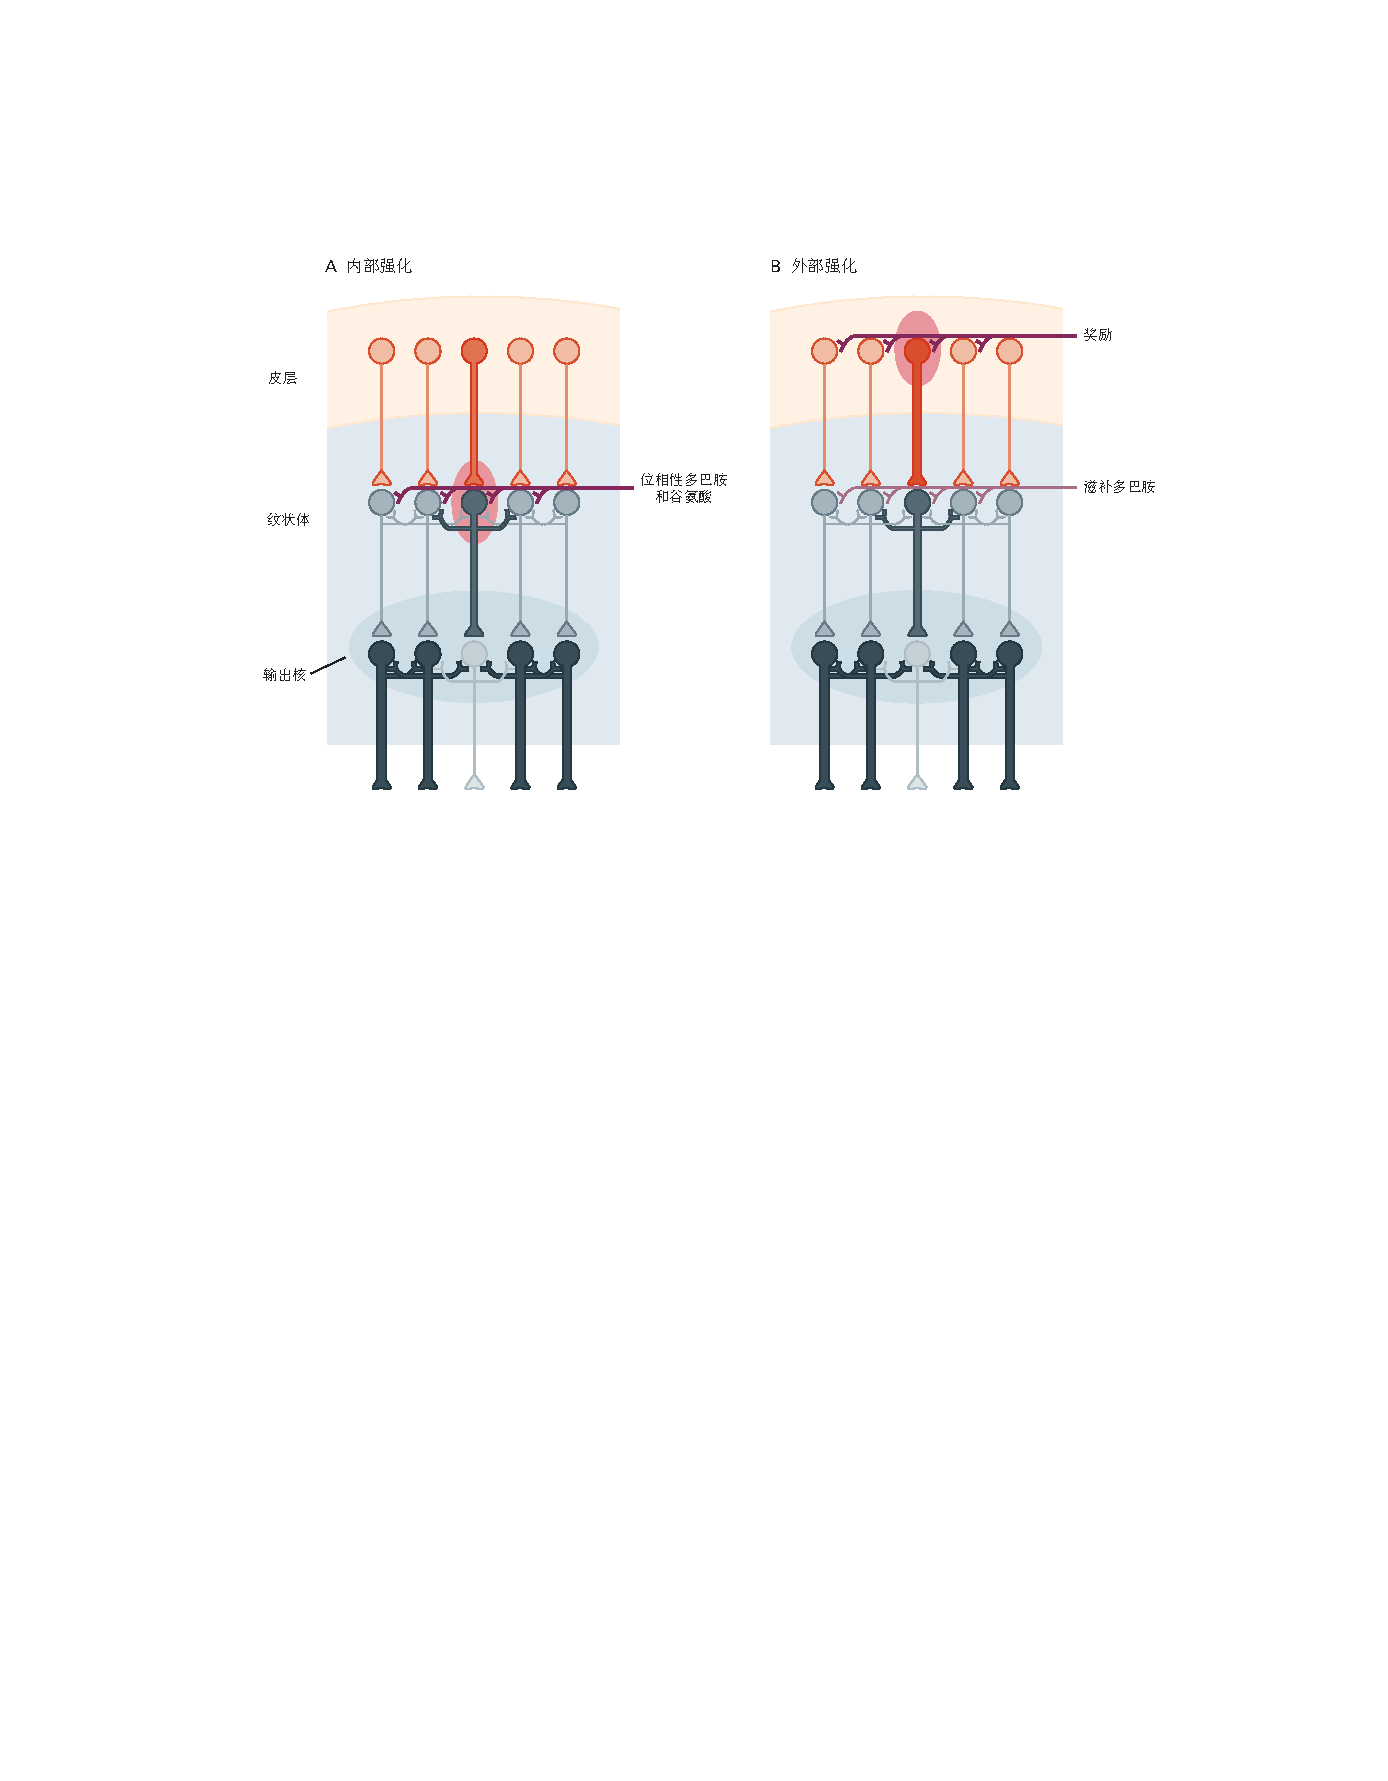
\includegraphics[width=1.0\linewidth]{chap38/fig_38_8}
	\caption{两个独立的强化机制可以在基底神经节的折返平行环结构中偏向选择。
		(为清楚起见,省略了通过丘脑的回路的返回连接。)
		\textbf{A.} 内在强化(红色椭圆形)涉及皮层纹状体神经传递的选择性敏化(由不同通道中纹状体投射神经元的相对厚度表示)。
		最近活跃的(选定的)通道中的传输通过多巴胺和谷氨酸的联合阶段性释放得到加强,该释放是由不可预测的生物学显著感觉事件(例如奖励)引起的。
		非活动通道缺乏突触多巴胺强化所需的资格跟踪。
		由此产生的选择性可塑性将导致优先重新选择近期行为输出的强化版本,从而在行动和结果之间建立关联。
		\textbf{B.} 最近的研究表明,与奖励(红色椭圆形)的关联可以加强向纹状体提供传入信号的结构中的处理。
		就基底神经节的选择部分取决于输入到纹状体(共同货币)的相对强度而言,传入信号的奖赏相关调制将有效地使选择偏向于奖赏相关输入。
		同样,图中投影的粗细表示激活的相对水平。}
	\label{fig:38_8}
\end{figure}



\subsection{内部强化是由基底神经节核内的相位多巴胺信号调制的}

基底神经节强化的流行观点是,动作选择受到多巴胺教学信号的影响,该信号调整内在回路的敏感性,从而增强对与不可预测的奖励相关的输入的反应(图~\ref{fig:38_8}A)。
因此,在这个模型中,强化学习过程是基底神经节核的固有过程。
然而,正如我们在上面看到的,多巴胺能神经元具有高度发散的轴突,这些轴突终止于目标细胞核的广泛区域。
再加上体积传递的问题,以及多巴胺能神经元通常作为一个整体对相关事件做出反应的事实,以及如何仅强化那些与奖励或惩罚相关的元素的问题立即变得显而易见。


人们认为,这个问题是通过调用衰减资格迹的概念来解决的。
也就是说,与导致奖赏的动作相关的神经元群中的尖峰活动被认为会改变这些神经元的特定状态,使它们能够接受后来广泛传播的与奖赏相关的强化信号。
有证据表明该过程在基底神经节内运行。
因此,在大多数当代模型中,竞争行为选项由特定神经元表示,其活动可以通过传入多巴胺信号的阶段性增加或减少来加强。


由于行为实验已经确定,不可预测的奖励而非奖励本身对学习至关重要,因此多巴胺能神经元的相位响应特性引起了生物学和计算神经科学界的关注。
生物实验和计算分析的强大结合现在清楚地表明,中脑多巴胺能神经元的相位活动为强化学习提供了教学信号。


在记录腹侧中脑的多巴胺能神经元时,大多数研究向受试者(通常是猴子)提供奖赏或预测奖赏的中性刺激。
这些实验的结果表明,由意想不到的奖励或预测它们的刺激开始引起的阶段性多巴胺反应具有较短的反应潜伏期(刺激开始后约 100 毫秒)和持续时间较短(再次约 100 毫秒)。
结果表明,这些反应的强度受到一系列因素的影响,包括奖励的大小、可靠性和延迟奖励的程度。
重要的是,当中性刺激预测奖励时(如传统巴甫洛夫条件反射),阶段性多巴胺反应从奖励转移到预测刺激。 或者,如果预测到奖励但未交付,则多巴胺能神经元会在奖励已交付时短暂暂停。
一个特别令人兴奋的发现是,这些响应类似于机器学习强化算法中的奖励预测误差项。
因此,人们普遍认为,阶段性多巴胺反应可以作为大脑在强化学习中的教学信号。


随着光遗传学方法的出现,现在已经毫无疑问地确定,阶段性多巴胺反应可以发出正面和负面奖励预测错误的信号,并且这些反应相应地增加和减少了选择先前行为的可能性。
据认为,阶段性多巴胺通过加强对纹状体中直接通路神经元的输入并削弱对间接通路神经元的输入来起作用。
因此,有证据表明直接通路活动可以导致动物做更多的特定动作,而间接通路活动会导致动物不做某项动作。


然而,这些途径的作用可能比这种简单的二分法更复杂。
根据上面概述的不同行动维度(什么、哪里、何时以及如何),直接和间接途径中的活动可以加强或阻止更快或更慢的运动,具体取决于在该情况下哪些运动会导致奖励。
此外,这些通路的光遗传学自我刺激对动作强化的影响似乎在纹状体的联合(背内侧)和感觉运动(背外侧)区域之间是不同的。
这可能与在腹侧被盖区观察到的不同多巴胺信号一致,腹侧被盖区在纹状体中向内侧突出,而在黑质致密部则向外侧突出。
后者具有更高比例的多巴胺能神经元,这些神经元对刺激显著性有反应,并优先在动物开始自定节奏的运动时做出反应(例如,在需要时按下杠杆获取食物,而不是在出现感官提示时)。


尽管如此,大量实验数据表明,基底神经节中多巴胺诱发的阶段性神经可塑性可以根据预测结果的值来偏向未来的行为选择。
这一结论与基底神经节作为支持强化学习的通用选择机制运作的观点一致。



\subsection{\textit{外部强化}可以通过在传入结构中操作来偏向选择}

第二种在可重入循环架构中导致偏向选择的机制不太为人所知,它是通过调节之前与强化物相关的竞争行为选项的输入显著性:奖励或惩罚(图~\ref{fig:38_8}B)。
由于竞争渠道中输入显著性的相对大小是判断竞争选项的通用货币,强化诱导增强特定渠道对选择机制的输入将增加该选项在未来被选中的可能性。


文献中的证据表明,当特定刺激与奖赏相关时,它在许多投射到基底神经节的传入结构中的表现得到增强。
在输入结构中调制处理的增强信号的来源目前未知。
然而,通过与奖励相关联的基底神经节输入预调整意味着与高价值结果相关的选项将具有相应更高的被选中概率。
通过奖励和惩罚不断更新输入显著性会使选择产生偏差,从而在长期内最大化获得奖励(或避免惩罚)。
最后,可能是与奖赏相关的对腹侧中脑传入输入的调整使多巴胺能神经元能够准确报告奖赏预测错误。


总之,强化学习很可能是选择架构的一个额外的固有属性。
平行可重入循环体系结构周围不同位置的突触中继点为特定循环中的活动提供了充分的机会,可以通过奖励和惩罚来调节。
现在有充分的证据表明,选择偏差可以通过涉及基底神经节内多巴胺广泛释放的机制通过奖励来实现。
强化选择性很可能通过某种形式的资格机制来实现。
第二种可能性是,行为选择的相对显著性可以通过直接作用于向基底神经节提供输入的结构内的奖励和惩罚来调节。



\section{基底神经节的行为选择受目标导向和习惯控制}

在过去的几十年里,很明显,可以学习行动,然后根据目标导向或习惯性控制来选择行动。
最初,当我们学习执行特定行动以获得特定结果时,这些行动是目标导向的,并且它们的表现对结果预期值的变化或行动与结果之间的偶然性变化高度敏感。
通过重复和巩固,行动不仅可以变得更有效率,而且可以更加自动化,由刺激-反应型回路控制。


就习惯而言,绩效对结果价值的变化或行动与结果之间的偶然性变化变得不那么敏感,而是受到先行刺激或背景的显著性的控制。
有趣的是,从目标导向行为到习惯行为的转变不仅可以通过延长训练来实现,还可以通过不同的强化计划来实现。
因此,当根据随机时间间隔提供奖励时,有利于习惯的形成,而当在随机数量的动作后提供奖励时,有利于目标导向控制。


不同的皮层-基底神经节环路似乎支持目标导向行为与习惯的学习和表现。
目标导向动作的获得似乎依赖于涉及背内侧或关联纹状体、前边缘皮层、内侧丘脑、眶额皮层和杏仁核的关联皮质-基底神经节回路。
另一方面,习惯的形成取决于通过背外侧或感觉运动纹状体、边缘下皮层和中央杏仁核的回路。


已经表明,由于这两种基本的行为控制模式通过不同的重入环路运行,因此有可能通过基底神经节内的特定操作引起它们之间的转换。
因此,联合区域的损坏或失活有效地阻止了目标导向的控制,同时使自动习惯性控制相对未受损。
相反,感觉运动基底神经节的破坏会导致习惯性表现切换回目标导向控制。


最后,有效的习惯,即已知的刺激或环境会触发特定的反应,在日常生活中非常有用,例如系鞋带或锁前门。
然而,我们也会遇到使我们重新评估我们的行为的情况。
在目标导向的行为和习惯之间转换使我们能够在环境中灵活地行动,而不能这样做可能是在成瘾和基底神经节的其他行为和神经障碍中观察到的扭曲行为的基础。
我们现在转向这个话题。



\section{基底神经节疾病可能与选择障碍有关}

本章的重点是基底神经节的功能结构及其进化历史如何决定它们在整体大脑功能中的作用。
我们所有人进行这项练习的动机之一是试图理解我们目前不了解的事物的内在科学兴趣。
然而,还有另一个重要原因需要更好地了解基底神经节的运作方式。
在人类中,基底神经节功能障碍与许多使人衰弱的疾病有关,包括帕金森病、亨廷顿病、图雷特综合症、精神分裂症、注意力缺陷障碍、强迫症和许多成瘾症。
许多研究试图阐明基底神经节功能障碍如何导致这些疾病的特征性症状。
只有当我们更好地了解像基底神经节这样的复杂系统在正常运行时试图做什么时,这种努力才会有所帮助。



\subsection{选择机制可能容易受到多种潜在故障的影响}

到目前为止,我们已经考虑了支持基底神经节环路作为通用选择机制的观点的理论和经验证据,强化学习在其中运作以最大化奖励和最小化惩罚。
如果动作选择和强化学习是基底神经节的正常功能,那么应该可以根据选择或强化功能障碍来解释许多人类基底神经节相关疾病。


正常选择要求所选选项在基底神经节输出水平上解除抑制,同时保持或增加对未选择或丢失选项的抑制(图~\ref{fig:38_9}A)。
如果没有一个选项能够实现足够的去抑制以达到关键选择阈值(图~\ref{fig:38_9}B),那么这种系统中的一个明显失败就是。
然而,在考虑选择故障时,更重要的一点是要认识到输出抑制和去抑制可能是连续可变的,而不是离散的开/关状态。
在那种情况下,去抑制和抑制通道之间的差异将决定选择的“硬”或“软”程度。
当差异很大时(图~\ref{fig:38_9}D),竞争选项可能会发现当前选择具有抗干扰性,需要比正常输入更大的显著性才能使系统切换选择。
相反,当差异较小时(图~\ref{fig:38_9}C),竞争选项启动选择开关会相对容易。


\begin{figure}[htbp]
	\centering
	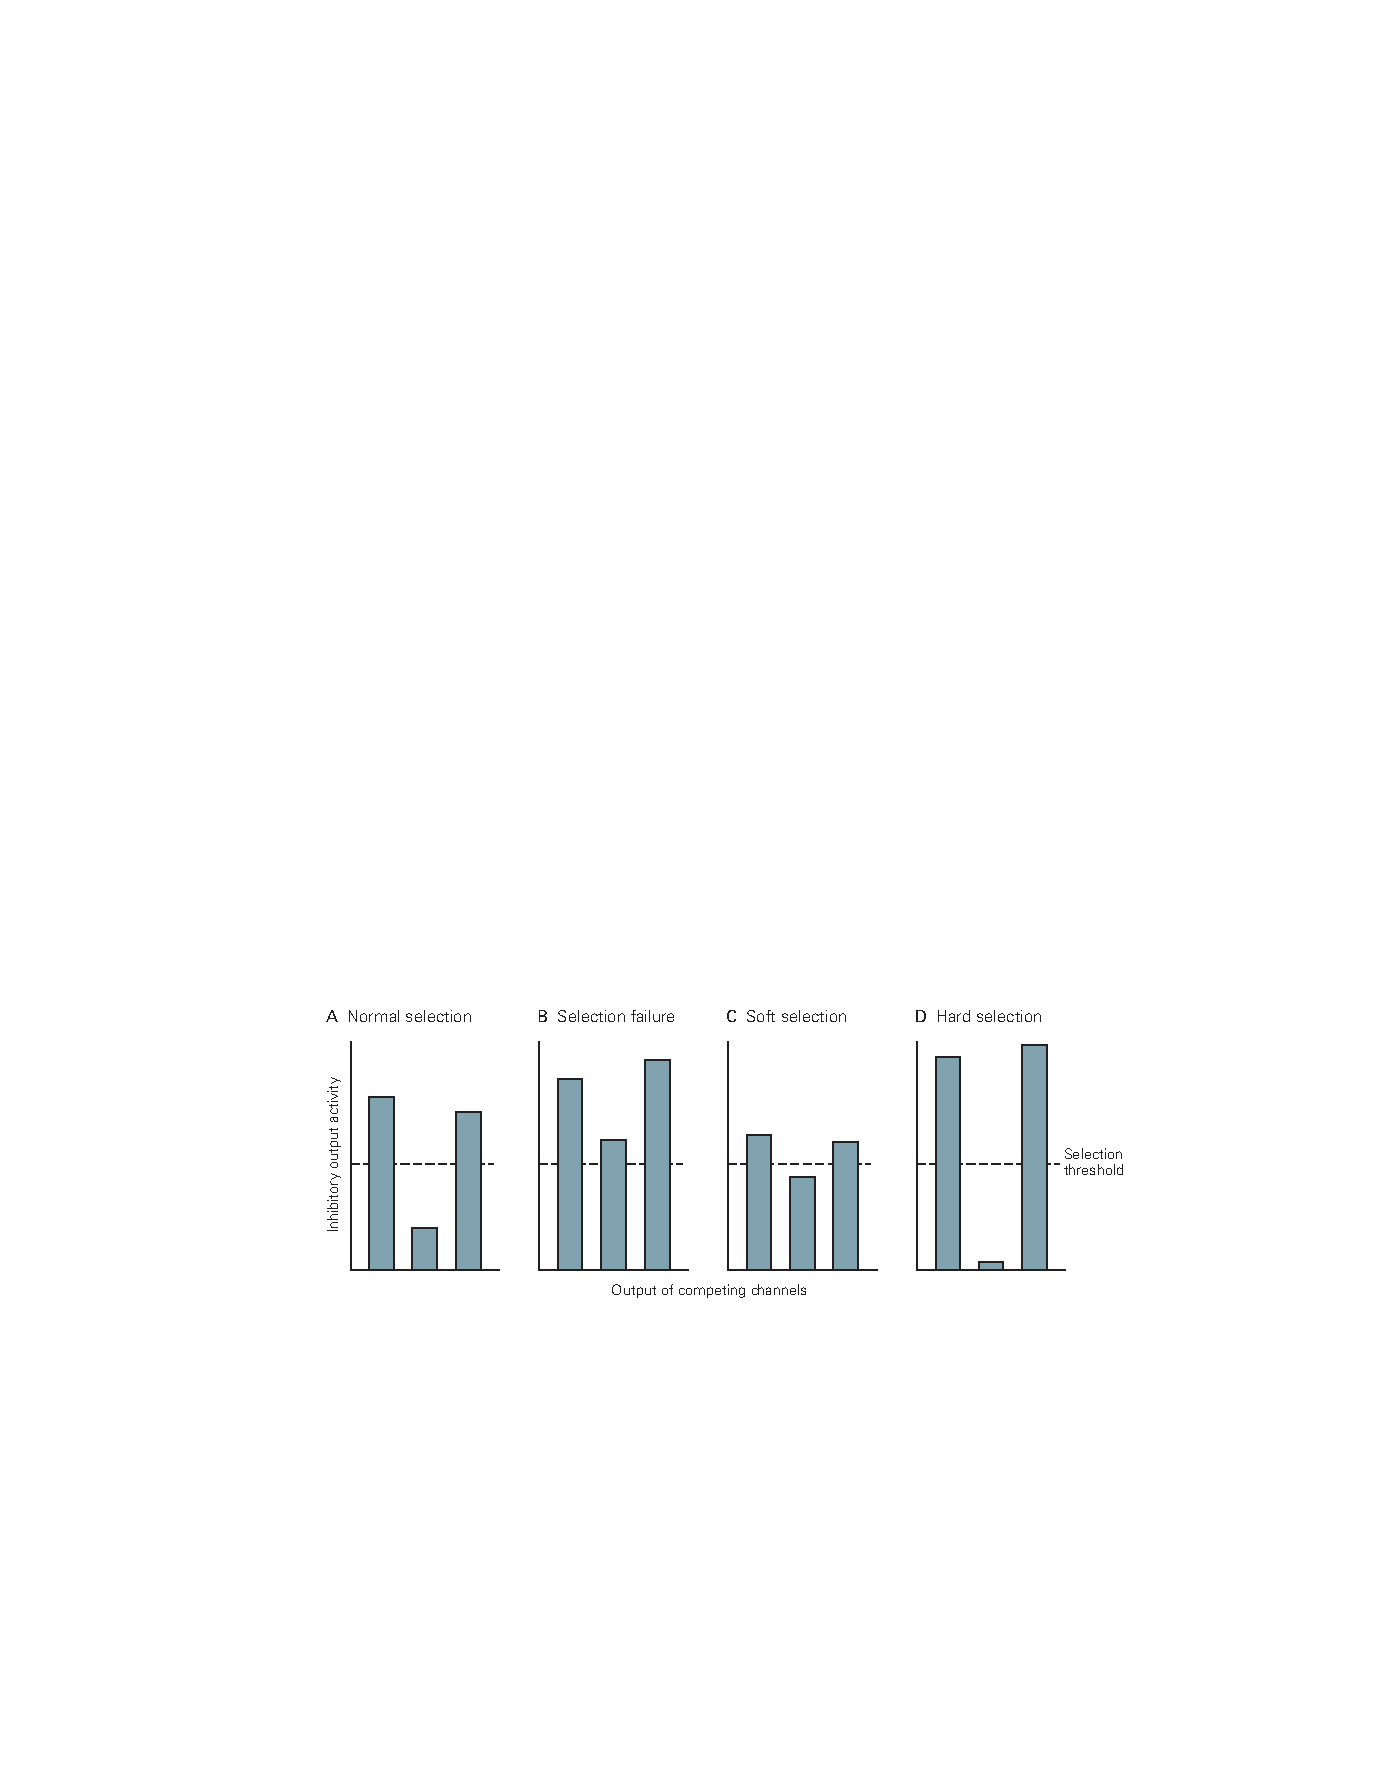
\includegraphics[width=0.92\linewidth]{chap38/fig_38_9}
	\caption{潜在的行为选择障碍。
		\textbf{A.} 基底神经节内的\textit{正常选择}的特点是对低于建议\textit{选择阈值}(中央通道)的选定通道的抑制减少,同时维持或增加对非选定通道(左右通道)的抑制。
		因此,去抑制的目标结构能够启动它控制的动作,而未选择的目标则保持在抑制控制之下。
		\textbf{B.} 所有通道的强直抑制减少不足意味着没有目标结构会被充分解除抑制。
		这种情况可以解释帕金森病的运动不能。
		\textbf{C.} 未能充分抑制所选通道或抑制竞争通道中的抑制活动会导致当前选择容易受到干扰。
		这种障碍可以解释精神分裂症和注意力缺陷多动障碍患者无法保持思路和容易因无人注意的事件而分心的原因。
		\textbf{D.} 一个通道可能通过所选通道的异常解除抑制或竞争通道的过度强直抑制而成为病理优势。
		这将使相关选项易于选择并且高度抗干扰。
		艰难的选择可以解释强迫症和成瘾行为。}
	\label{fig:38_9}
\end{figure}


对这些想法的支持来自行为观察,表明在任务学习开始时,策略之间经常很容易切换。
然而,随着任务的深入学习,系统对替代策略的抵抗力越来越强。
因此,在思考选择机制在基底神经节疾病的背景下如何变得功能失调时,理解硬选择和软选择的概念可能会发挥重要作用。



\subsection{帕金森病可以部分地视为未能选择感觉运动选项}

帕金森病的主要症状是运动不能(开始运动困难)、运动迟缓(开始运动缓慢)和僵硬(僵硬和对被动运动的抵抗)。 震颤经常但不总是存在。
导致帕金森病运动症状的主要神经缺陷被认为是基底神经节中多巴胺能神经传递的进行性退化。


这种多巴胺损失的结果是基底神经节输出核记录中的强直和振荡活动增加。
由于基底神经节的输出是\textit{$\gamma$-氨基丁酸}能和抑制性的,因此在帕金森病中,目标结构正在接受高水平且不均匀的抑制输入。
这种情况会损害基底神经节的正常选择性(去抑制)功能; 动作很难选择,而且在可能的情况下执行起来也很慢。


然而,帕金森病比这更微妙。
在这种进行性病症的大部分时间里,多巴胺能传递的丧失对基底神经节的感觉运动区域有不同的影响,而边缘和联想区域相对不受影响。
正如目标导向和习惯性控制部分所讨论的,基底神经节的感觉运动区域在选择习惯性行为中起着至关重要的作用。
因此,帕金森病的许多运动特征可以用自动习惯的丧失来解释,这也许并不奇怪。
虽然患者可以做事,但他们被困在目标导向控制的缓慢、连续和自愿模式中。
在未来,看看是否可以在临床症状出现之前检测到习惯性控制的细微丧失,从而作为该病症的早期标志物,将会很有趣。



\subsection{亨廷顿病可能反映了直接通路和间接通路之间的功能失衡}

亨廷顿病是一种遗传性疾病,最初的症状是情绪、性格、认知和身体技能的细微变化。
异常运动的特点是不稳定、随机和无法控制的运动,称为舞蹈病。
该疾病与神经元变性有关。
早期损伤在纹状体中棘神经元中最为明显,但随后会扩散到神经系统的其他区域。


观察到在纹状体的边缘、联想和感觉运动区域中神经元变性很明显,这可以解释为什么这种疾病的特征是情感、认知和感觉运动功能的紊乱。
同样值得注意的是,最脆弱的神经元是纹状体中投射到外部苍白球(间接通路)的神经元,而不是直接投射到基底神经节输出核的神经元。
在输出核的水平上,这种干扰会使平衡倾斜,有利于负责解除抑制的纹状体投射。
因此,亨廷顿舞蹈症的症状可能反映了未充分抑制的竞争者对所选情感、认知和感觉运动行为表达的干扰。



\subsection{精神分裂症可能与抑制非选择选项的普遍失败有关}

精神分裂性精神病是一种同时存在情感、认知和感觉运动功能障碍的病症。
典型症状包括妄想(不基于现实的错误信念)、幻觉(听到或看到不存在的事物)、思维混乱(从混乱的言语推断)和异常的运动行为(不可预测的激动、刻板印象和无法集中注意力 手头的事)。
该疾病是进行性的,在后期阶段,以情绪低落、社交退缩、思维缺失和运动行为减少为特征的阴性症状变得明显(第~\ref{chap:chap60}~章)。


由于许多不一致的实验程序、症状的高度可变性、药物的副作用、药物滥用以及对治疗的反应的可变性,理解精神分裂症的神经生物学基础变得复杂。
然而,就一类主要的抗精神病药物抑制多巴胺能神经传递而言,精神分裂症和基底神经节之间存在一致的联系。
就轴突末端和突触后多巴胺受体的简单区域密度而言,基底神经节内的多巴胺能传递可能受到多巴胺相关药物治疗的最深远影响。
此外,有证据表明基底神经节中的多巴胺失调是精神分裂症病理学的固有特征,而不是药物副作用;
早于精神病;
并且是疾病的危险因素。
这里的含义是精神分裂症与基底神经节中多巴胺能传递的净过量有关。


那么这种形式的失调会如何扭曲选择和强化的正常功能呢?
首先,精神分裂症以情感、认知和感觉运动行为障碍为特征的观察再次表明,神经生物学底物将存在于基底神经节的每个功能区。
其次,一个反复出现的主题是,随着阳性症状,似乎一切都太多了:强烈的情绪入侵、太多失控的想法、自发的感官体验、太多分散注意力的刺激,以及不可预测的运动激动。
统一这一系列令人困惑的症状的一种方法是假设它们代表了在基底神经节的不同功能区域中出现的类似基本故障。
在这里,基本故障可能是负责抑制竞争但未选择的选项的影响的机制部分出现故障。
因此,在所有功能区域中,当前选择的选项在病态上容易受到干扰(图~\ref{fig:38_9}C)。



\subsection{注意缺陷多动障碍和图雷特综合症也可能以非选择性选项的侵入为特征}

与基底神经节功能障碍相关的过度活跃状况的其他例子也可能是由于错误的选择机制,在这种机制下,每种情况下的系统都容易受到入侵。
\textit{注意缺陷多动障碍}与精神分裂症一样,部分原因可能是负责抑制非选择性感觉选择的机制出现故障,从而难以保持注意力集中。
或者,这种情况的冲动方面可能反映了神经系统的故障,这些神经系统会根据可能后果的价值产生行为选择。
在这种情况下,由即时期望的感官事件驱动的选项将优先于不利的长期后果的竞争表示。


在\textit{图雷特综合症}的案例中,越来越多的证据表明,无意识的行为入侵(言语和运动抽搐)与皮层-基底神经节-丘脑环路的异常活动有关。
在动物模型中,可以通过阻断感觉运动纹状体局部区域的抑制性神经传递来诱发类似的运动抽搐。
如果疾病状态也会在未被当前选择参与的纹状体部分引起类似的抑制失败或不适当的兴奋,则可能会出现破坏性运动入侵。
此外,如果过度兴奋的轨迹保持不变,并且重复入侵的运动特征,则很可能会启动自动习惯建立机制,从而进一步增强入侵的自动非自愿性。



\subsection{强迫症反映了病态主导选项的存在}

强迫症患者强迫性地重复特定的动作(洗手、数数、检查东西)或不请自来地反复出现特定的想法(强迫症)。
当症状出现时使用功能性神经影像学的研究一致报告皮层-纹状体-丘脑皮层环内不同位置的异常激活。


在选择机制功能障碍方面,当无论出于何种原因,相关功能通道的输入显著性异常占主导地位时,就会出现强迫症的症状,从而使竞争选择难以中断或引起行为或注意力 切换(硬选择)。
强迫性和强迫性选项是已习得的主导行为这一事实表明,导致强迫症的错误可能在于能够调整输入显著性的强化机制。
当然,这样的故障可能是遗传和/或环境原因造成的。



\subsection{成瘾与强化机制和习惯性目标的紊乱有关}

吸毒成瘾和其他行为(例如,赌博、性、饮食)代表了动机选择的严重失调。
这是由与成瘾相关的刺激、暴饮暴食和戒断焦虑的过度显著引起的。
当获得成瘾时,已经报道了基底神经节中多巴胺能和阿片样肽传递的变化。


就这些传输系统与强化的基本机制相关联而言,可以预期与成瘾相关的刺激的选择性强化将导致观察到这些刺激捕获行为的能力增加。
或者,戒断期间负面情绪状态和压力样反应的增加与多巴胺功能的降低有关。
在基底神经节的边缘区域,这种减少通常与负强化有关。


最后要注意的一点是,如果与成瘾相关的刺激可以自动触发放纵的动机/目标(即自动刺激 - 目标关联),则可能会在边缘区域运行一种与目前分配给刺激的类似机制 – 感觉运动区域的反应习惯。
因此,如果在吸毒成瘾的情况下,获取药物的目标可以被正确地描述为刺激驱动的习惯,那么获取药物的实用性就可以是高度目标导向的(例如,抢劫便利店、给经销商打电话),而不是 完全习惯。


从以上部分可以看出,根据选择和强化失调来解释基底神经节疾病不需要难以置信的智力扭曲。
事实上,这可以被视为进一步支持基底神经节的系统级功能是作为通用选择机制运行的观点。
此外,拥有一个基于正常功能潜在障碍的首要概念框架对于指导未来的研究具有重要优势。
人们不是在患者和动物模型的大脑中寻找可能出错的线索,而是在特定网络中寻找可能会导致观察到的疾病的故障。



\section{要点}

1. 基底节是一组相互连接的核,位于前脑和中脑的底部。
存在三种主要的\textit{输入}结构(纹状体、底丘脑核和黑质的多巴胺细胞)和两种主要的\textit{输出}结构(内部苍白球和黑质网状部)。


2. 输入结构接收来自大脑皮层、边缘系统和脑干的大部分区域的投射,其中许多是通过丘脑中的中继进行的。
纹状体和底丘脑的输入是按地形组织的。


3. 空间地形图在整个内在基底神经节连接中保持不变,并在返回到皮层、边缘系统和脑干结构的投射中保持不变。
因此,系统级基底神经节架构的一个基本特征可以被视为一系列可重入循环。


4. 纹状体被认为通过直接和间接途径连接到输出核。
然而,最近的解剖学证据表明其内部结构更为复杂。


5. 基底神经节的相位兴奋性输入由神经递质谷氨酸介导。
来自基底神经节的强直抑制输出由神经递质\textit{$\gamma$-氨基丁酸}介导。
可重入环将传入结构保持在强烈的抑制控制之下。
对于任何任务,一些输出神经元的强直抑制性放电会暂停,而对于其他神经元,它会维持或增加。


6. 基底神经节结构出现在脊椎动物进化之初,并且自始至终都高度保守。
这表明它们解决的计算问题很可能是所有脊椎动物物种都面临的问题。


7. 内在基底神经节核的内部微结构在其动机、情感、认知和感觉运动区域中基本相同。
这表明相同的基底神经节算法适用于所有一般类别的大脑功能。


8. 基底神经节文献中反复出现的主题是它们参与动作选择和强化学习。


9. 选择假设得到以下支持:
(1)选择是所有脊椎动物都面临的普遍问题。
(2)所有基底神经节区域通用的选择算法可以解决不相容的动机、情感、认知和感觉运动选项之间的竞争。
(3)许多内在过程可以支持选择功能。
(4)在多重入环结构中选择性去除输出抑制必然是一个选择过程。
(5)基底神经节结构的计算模型有效地选择了多功能机器人的动作。 


10. 大量证据表明,基底神经节是强化学习的重要基质,在强化学习中,选择会因过去结果的效价/价值而产生偏差。


11. 行动的多维方面(做什么、在哪里、何时以及如何做某事)可以通过强化学习独立修改。
重要的是要确定这些不同方面的动作是在基底神经节的相同或不同功能区域内学习的。


12. 最近的光遗传学研究证实,相位多巴胺信号可以作为强化学习的训练信号。


13. 在可重入环结构中,未来的选择不仅会因多巴胺而偏向基底神经节,还会偏向外部传入结构和丘脑中继的突触。


14. 强化学习可以根据结果值(目标导向)或通过对获得的自动刺激-反应关联(习惯)进行操作来使选择产生偏差。
目标导向和习惯性选择是在基底神经节的不同功能区域进行的。


15. 就人类基底神经节疾病可以解释为选择障碍而言,基底神经节作为通用选择模块运作的观点提供了额外的支持。

